\documentclass[10pt, xcolor=x11names,compress]{beamer}
\usepackage{tabulary}
\usepackage{booktabs}
\usepackage{float}
\usepackage{graphicx}
\usepackage{mwe}% for example pictures
\usepackage{siunitx}
\usepackage{hyperref}

\definecolor{sangria}{rgb}{0.57, 0.0, 0.04}
\usecolortheme[named=sangria]{structure}
\useoutertheme{infolines}
\usefonttheme[onlymath]{serif}
\setbeamertemplate{headline}[default]
\setbeamertemplate{navigation symbols}{}
\mode<beamer>{\setbeamertemplate{blocks}[rounded][shadow=true]}
\setbeamercovered{transparent}
\setbeamercolor{block body}{use=structure, fg=white, bg=black!20}
\setbeamercolor{itemize item}{fg=black}
\setbeamercolor{itemize subitem}{fg=gray} 
\setbeamercolor{itemize subsubitem}{fg=black!20} 
\makeatletter\setbeamertemplate{footline}
{  
	\leavevmode%  
	\hbox{%  
		\begin{beamercolorbox}[wd=.333333\paperwidth,ht=2.25ex,dp=1ex,center]{author in head/foot}%    
			\usebeamerfont{author in head/foot}
			\insertshortauthor%~~\beamer@ifempty{\insertshortinstitute}{}
		\end{beamercolorbox}%  
		\begin{beamercolorbox}[wd=.333333\paperwidth,ht=2.25ex,dp=1ex,center]{institute in head/foot}%    
			\usebeamerfont{title in head/foot}\insertinstitute  
		\end{beamercolorbox}%  
		\begin{beamercolorbox}[wd=.333333\paperwidth,ht=2.25ex,dp=1ex,right]{date in head/foot}%    
			\usebeamerfont{date in head/foot}\insertshortdate{}\hspace*{2em}    
			\insertframenumber{} / \inserttotalframenumber\hspace*{2ex}   
	\end{beamercolorbox}}%  
	\vskip0pt%
}
\makeatother 
\useoutertheme[footline=empty, subsection=false]{miniframes}
\usepackage{multicol}  
\author{Núcleo de Estudos Raciais}
\title{Apresentação - Resultados Preliminares Carta de Conjuntura Mercado de Trabalho}

\institute{Insper}\date{10/07/2024} 
\begin{document}
	\begin{frame}
		\titlepage
	\end{frame}
	
	
	\section{Contexto} 
	\begin{frame}{Rendimento Recente do Trabalho}
	\begin{figure}
		\centering
		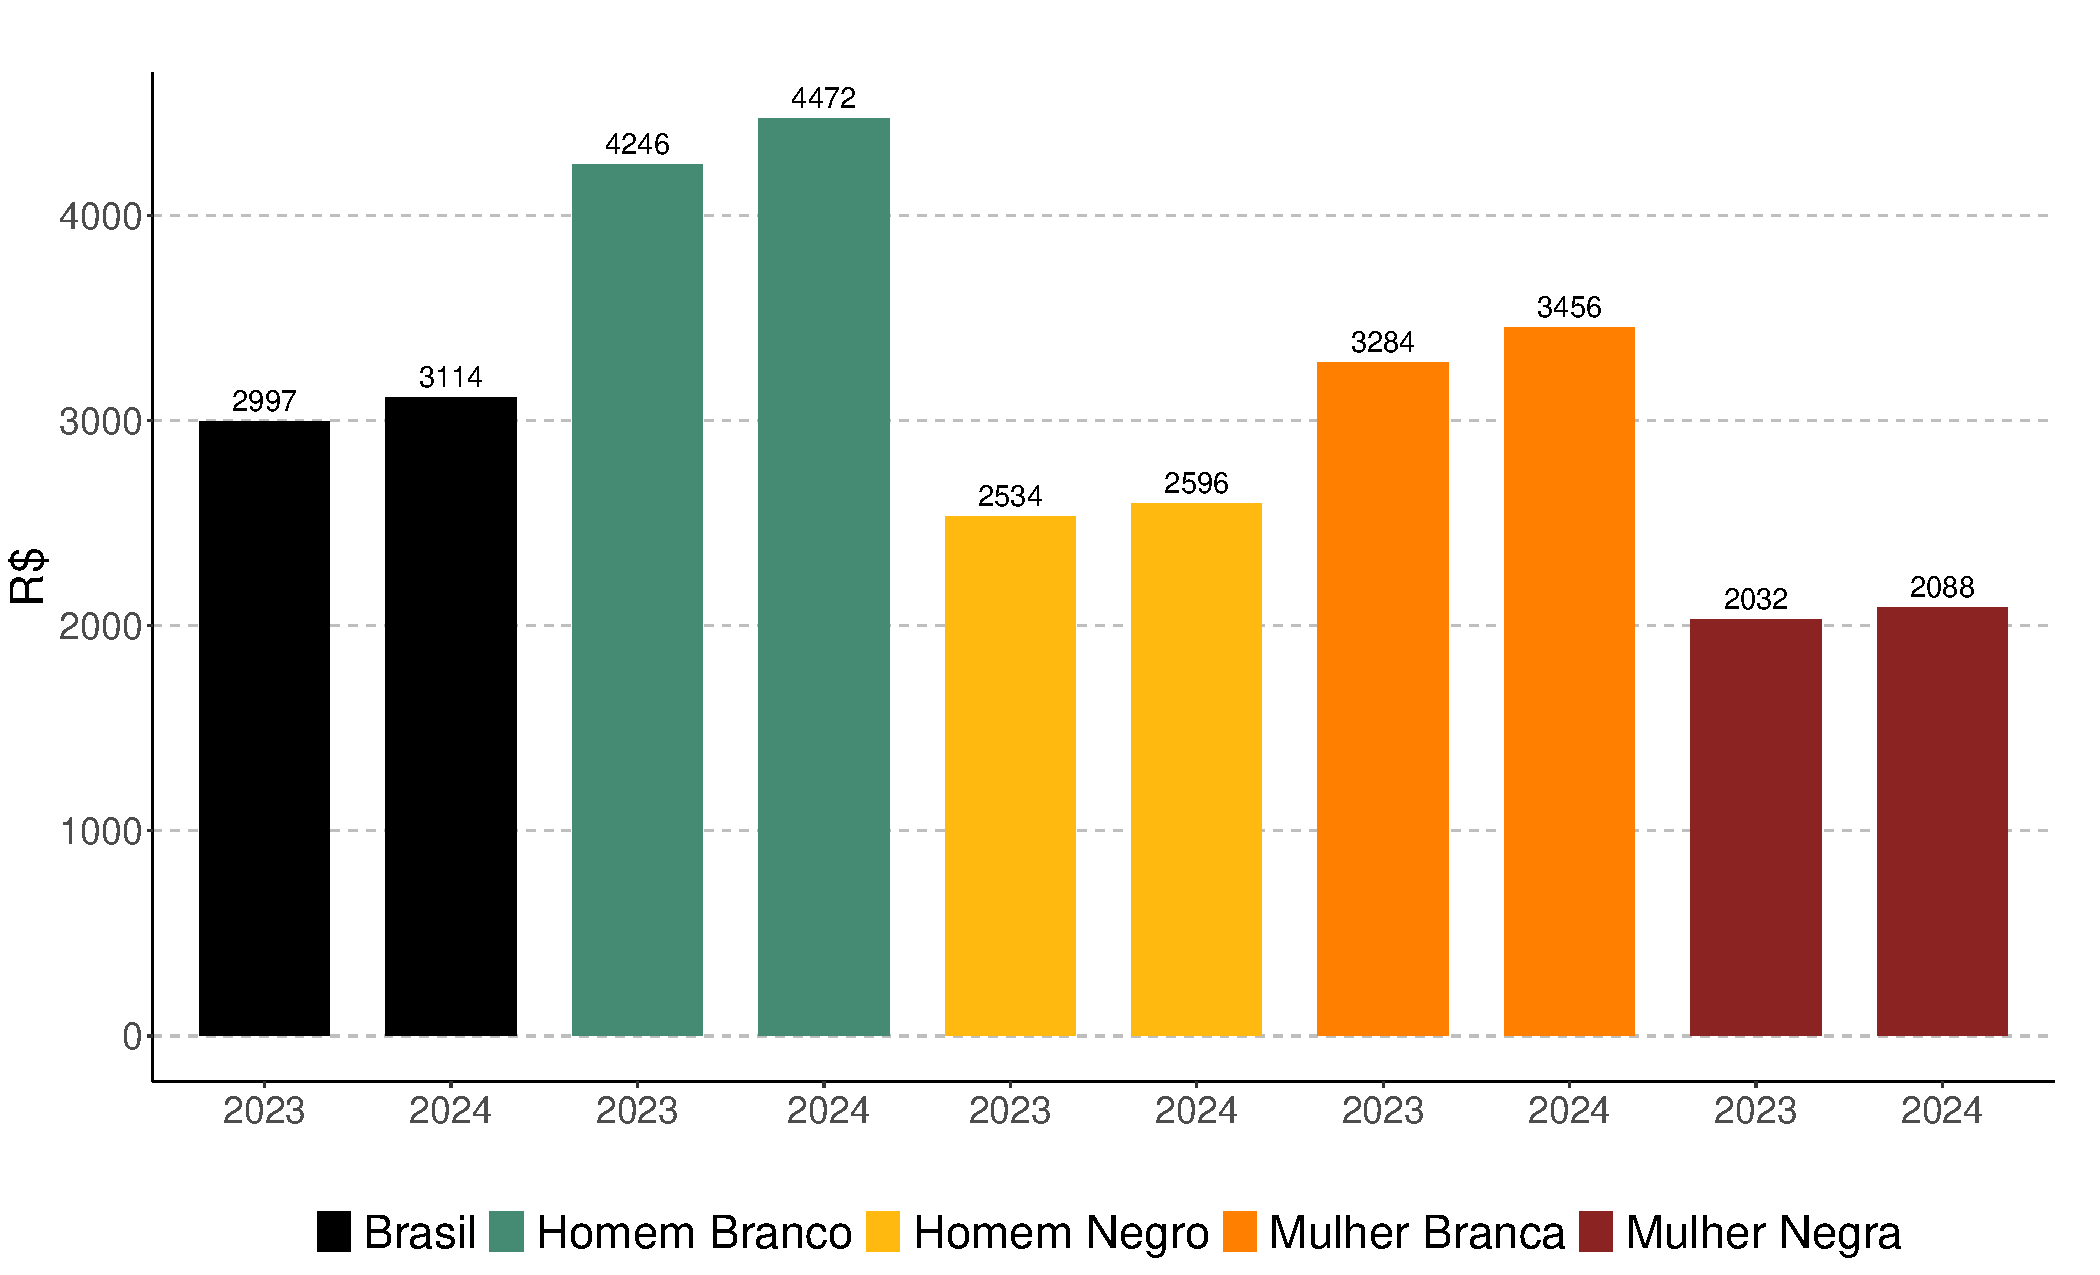
\includegraphics[width = 0.75\textwidth]{figures_output/rendimento_habitual.pdf}
	\end{figure}
	\end{frame}			
	
	\begin{frame}{Desigualdade Salarial}
	\begin{figure}
		\centering
		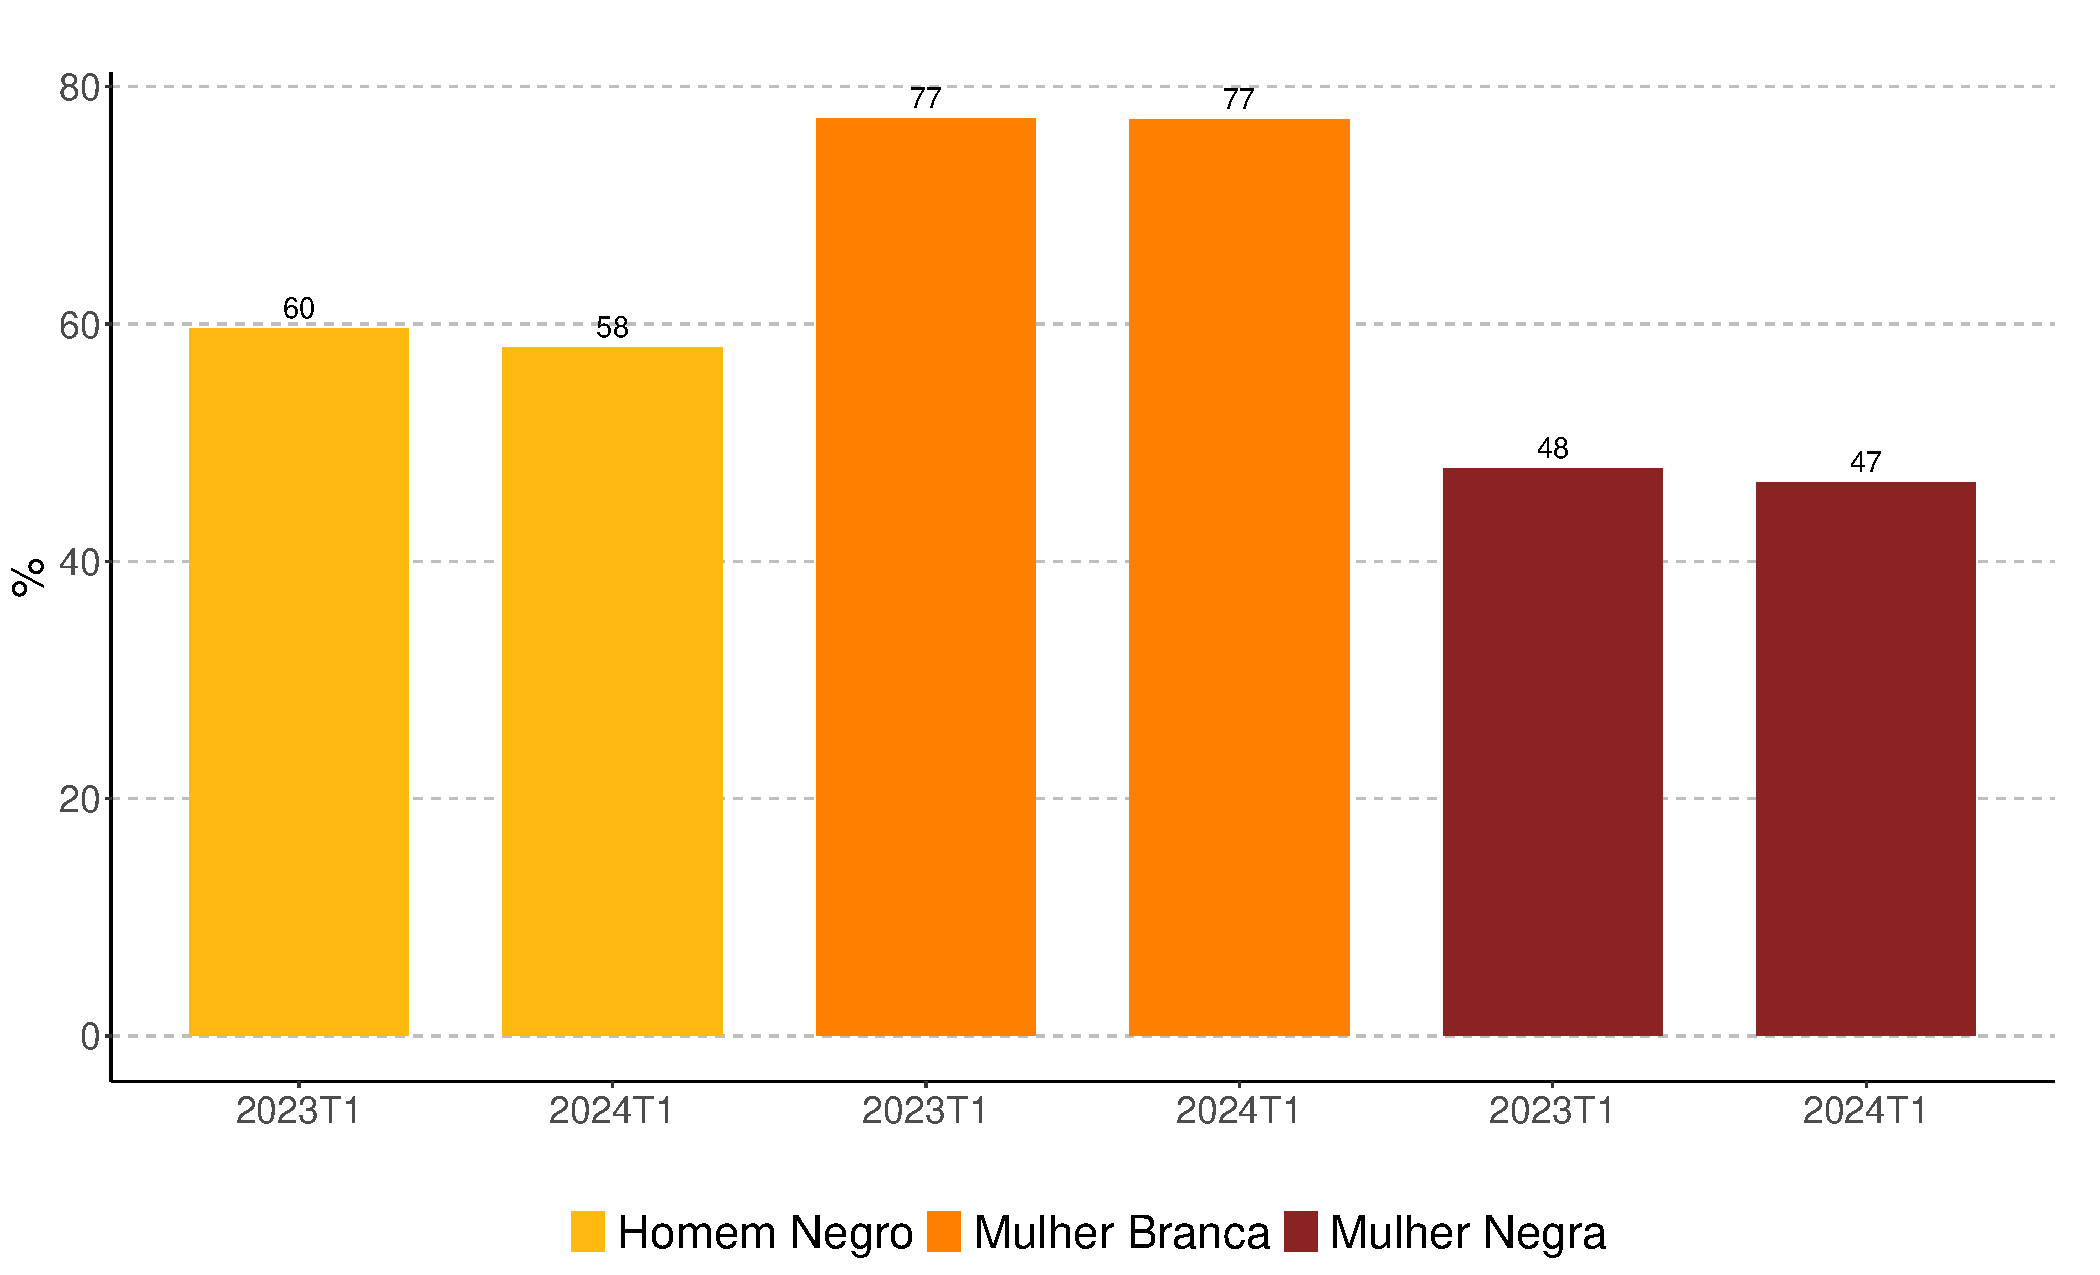
\includegraphics[width = 0.75\textwidth]{figures_output/frac_rendimento_habitual.pdf}
	\end{figure}
	\end{frame}			
	
		\begin{frame}{Rendimento Habitual Médio de Todos os Trabalhos}
		\begin{figure}
			\centering
			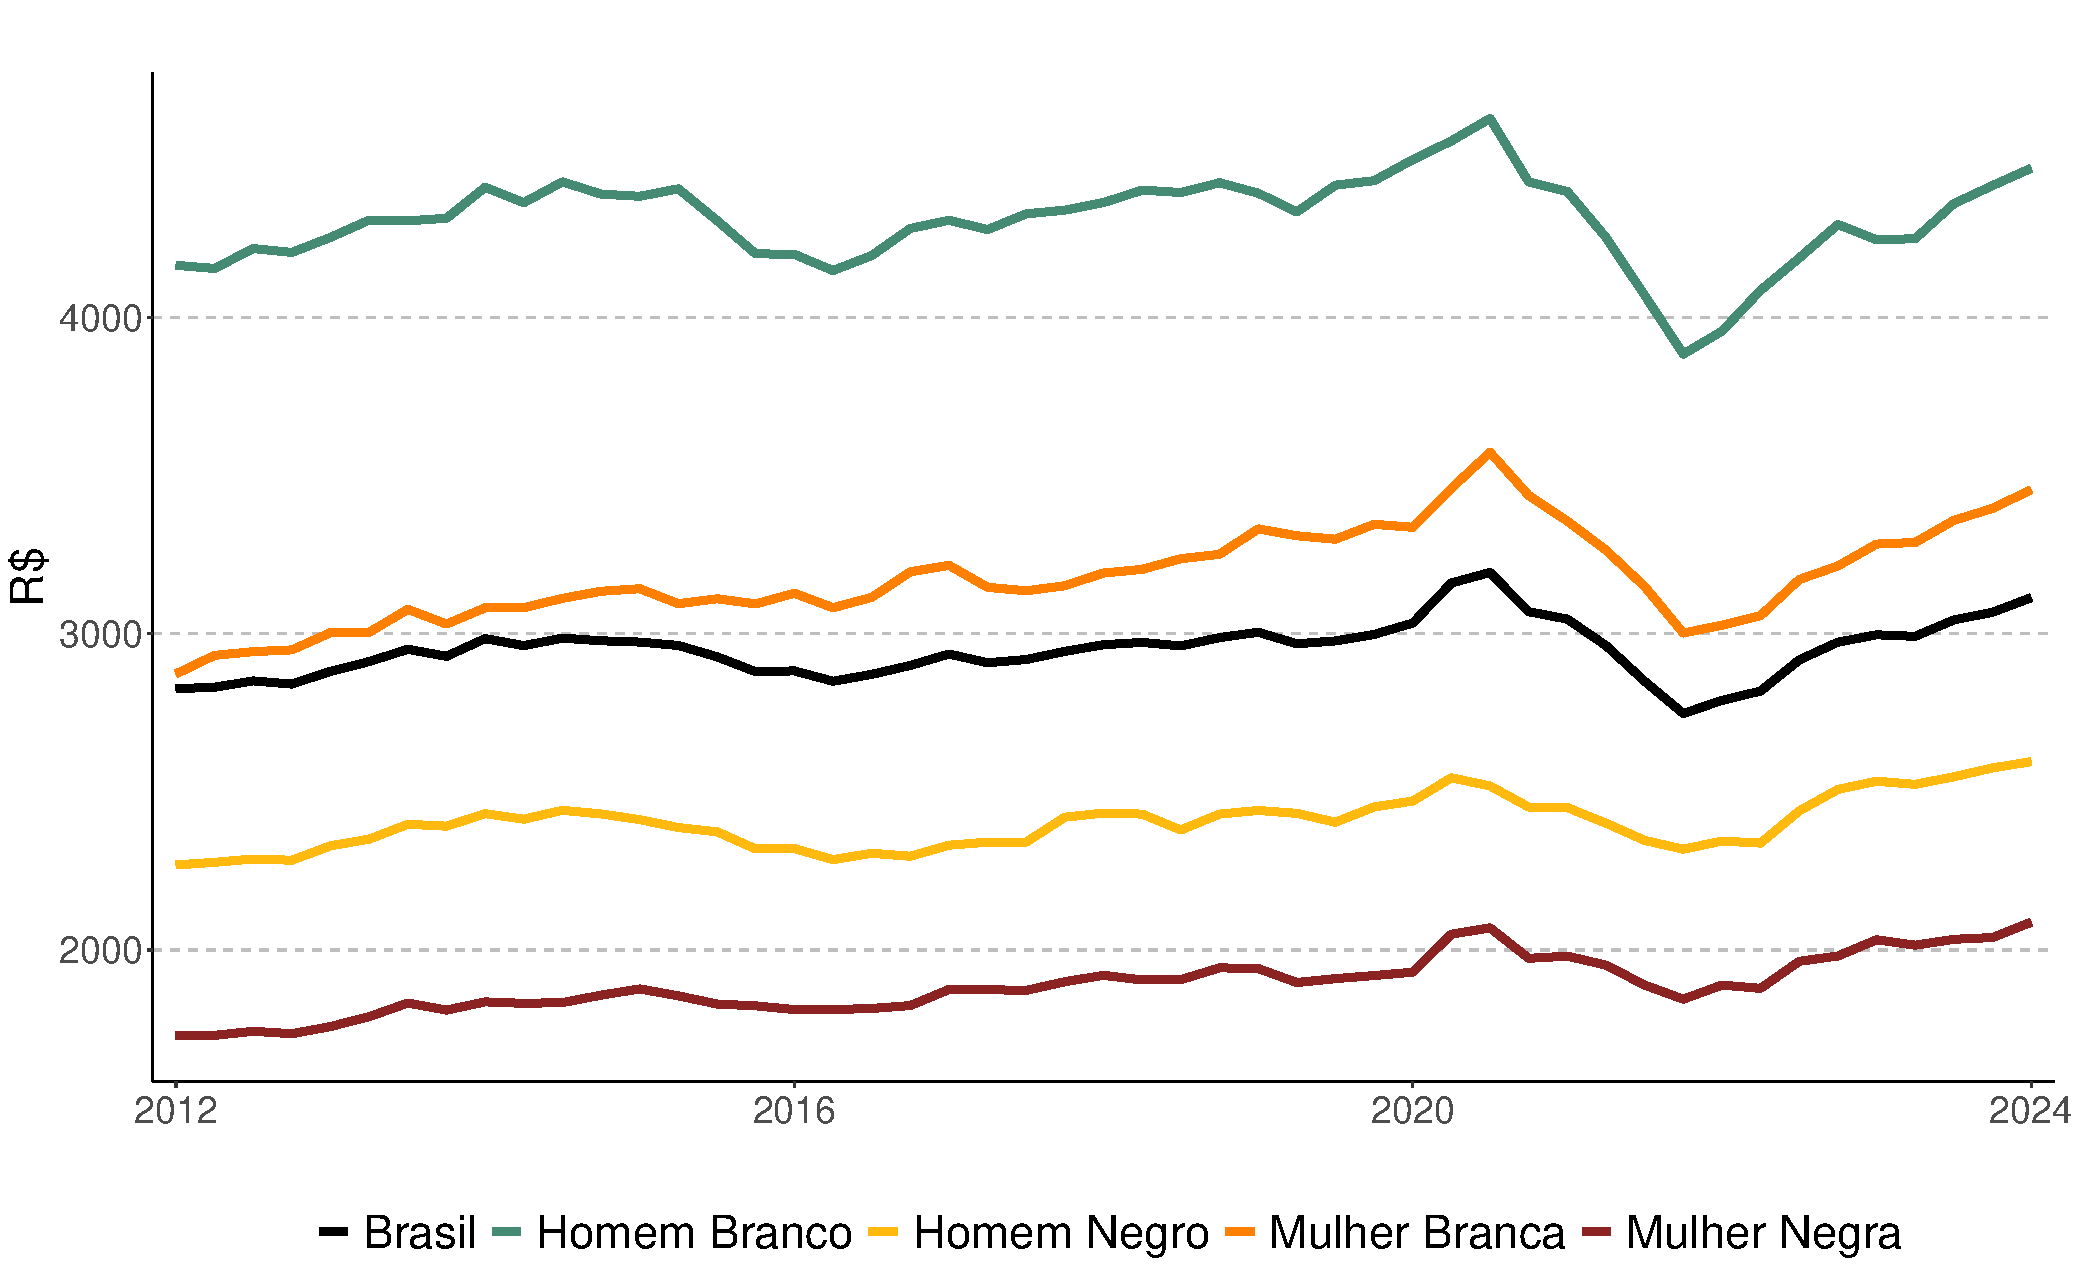
\includegraphics[width = 0.75\textwidth]{figures_output/rendimento_habitual_br_gen_raca.pdf}
		\end{figure}
	\end{frame}	
	
		\begin{frame}{Desemprego Recente}
		\begin{figure}
			\centering
			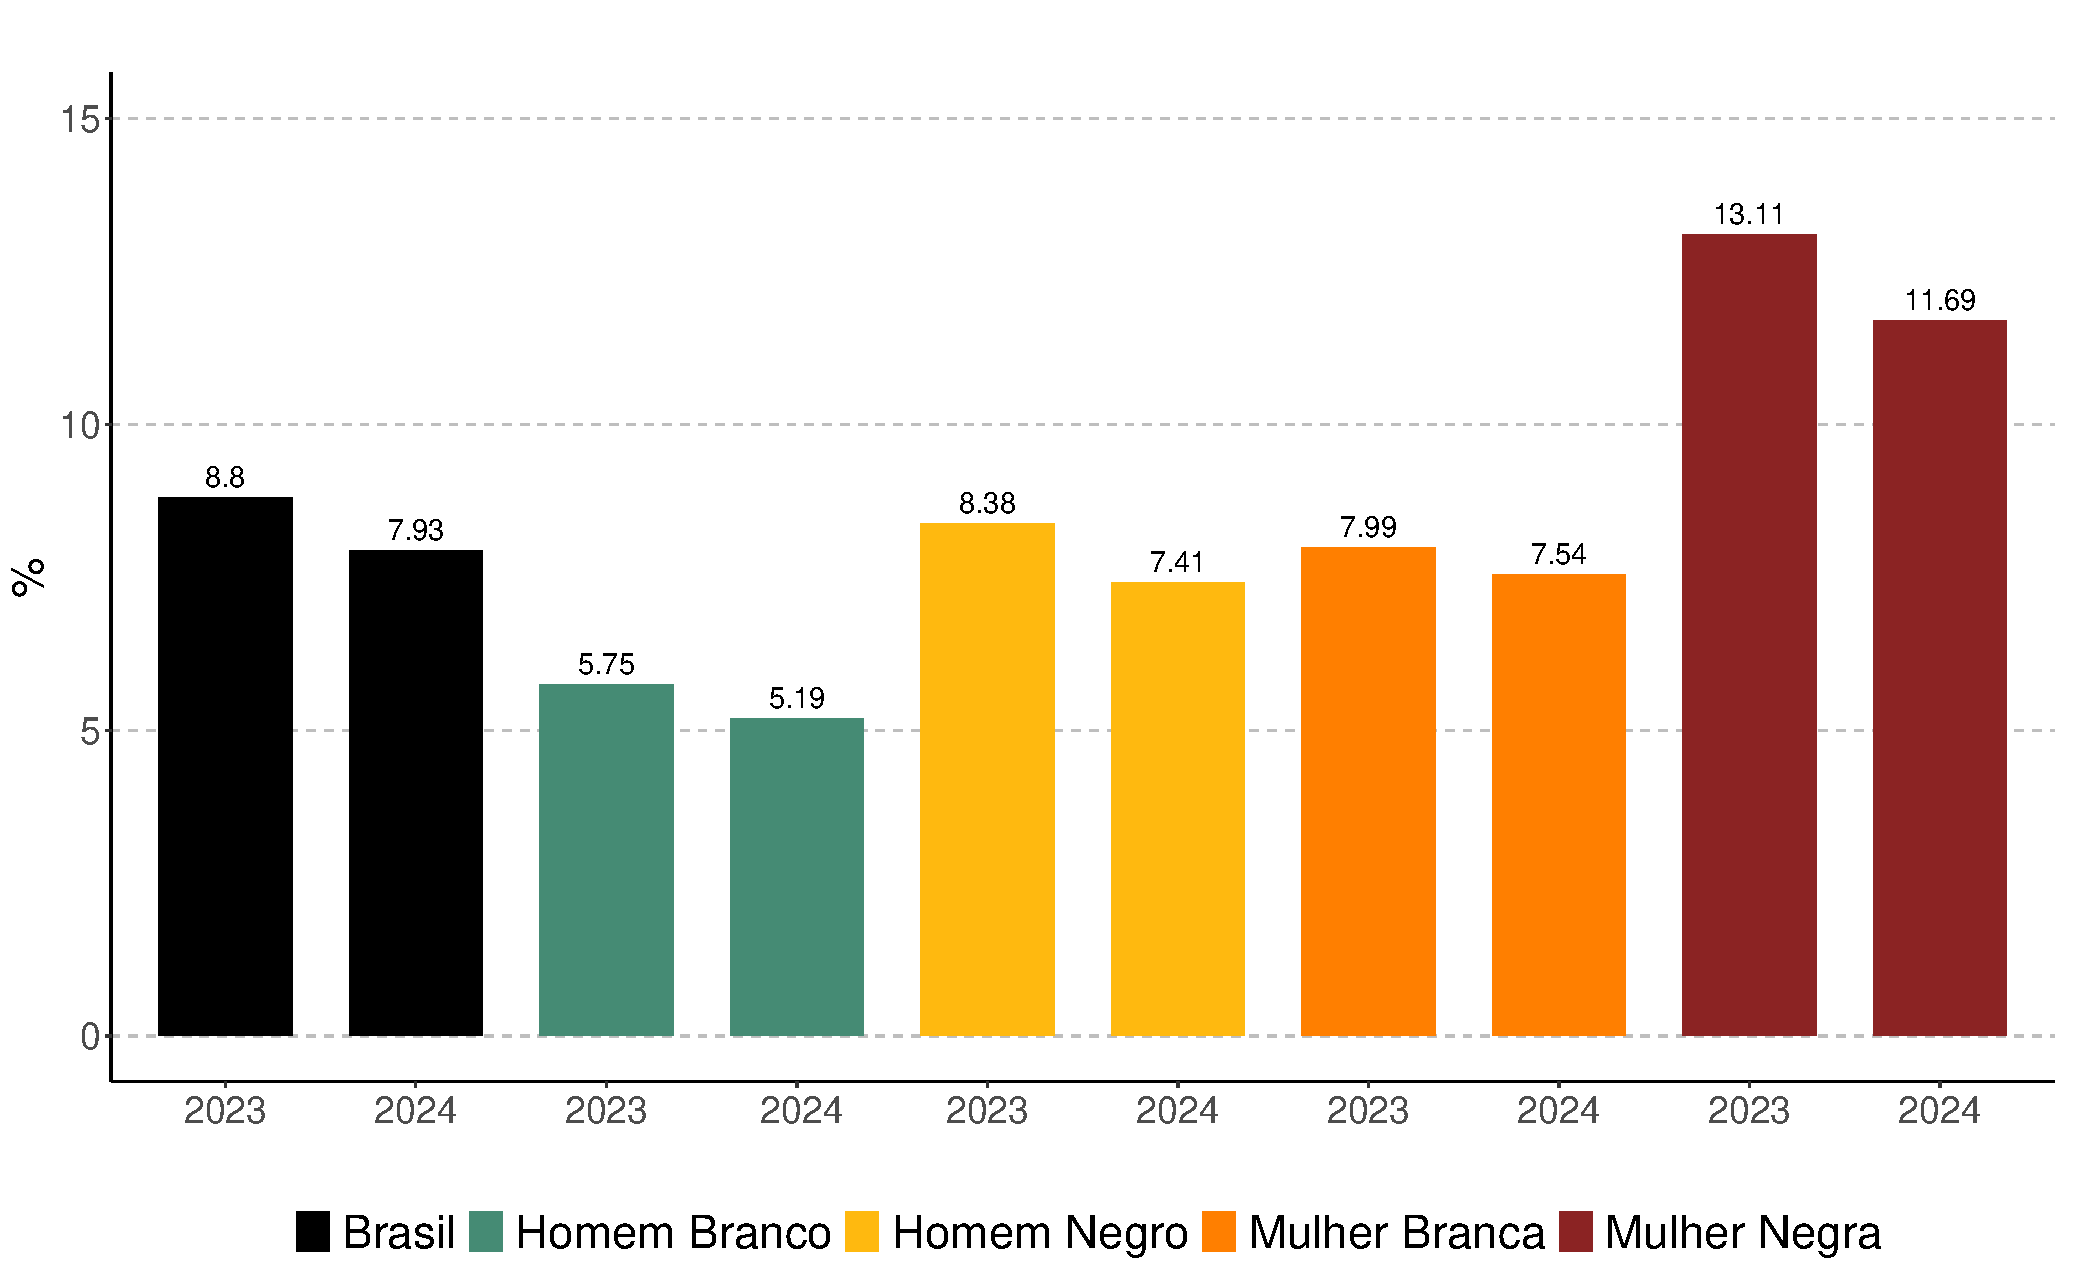
\includegraphics[width = 0.75\textwidth]{figures_output/unemp.pdf}
		\end{figure}
	\end{frame}
	
		\begin{frame}{Desigualdade no Desemprego}
		\begin{figure}
			\centering
			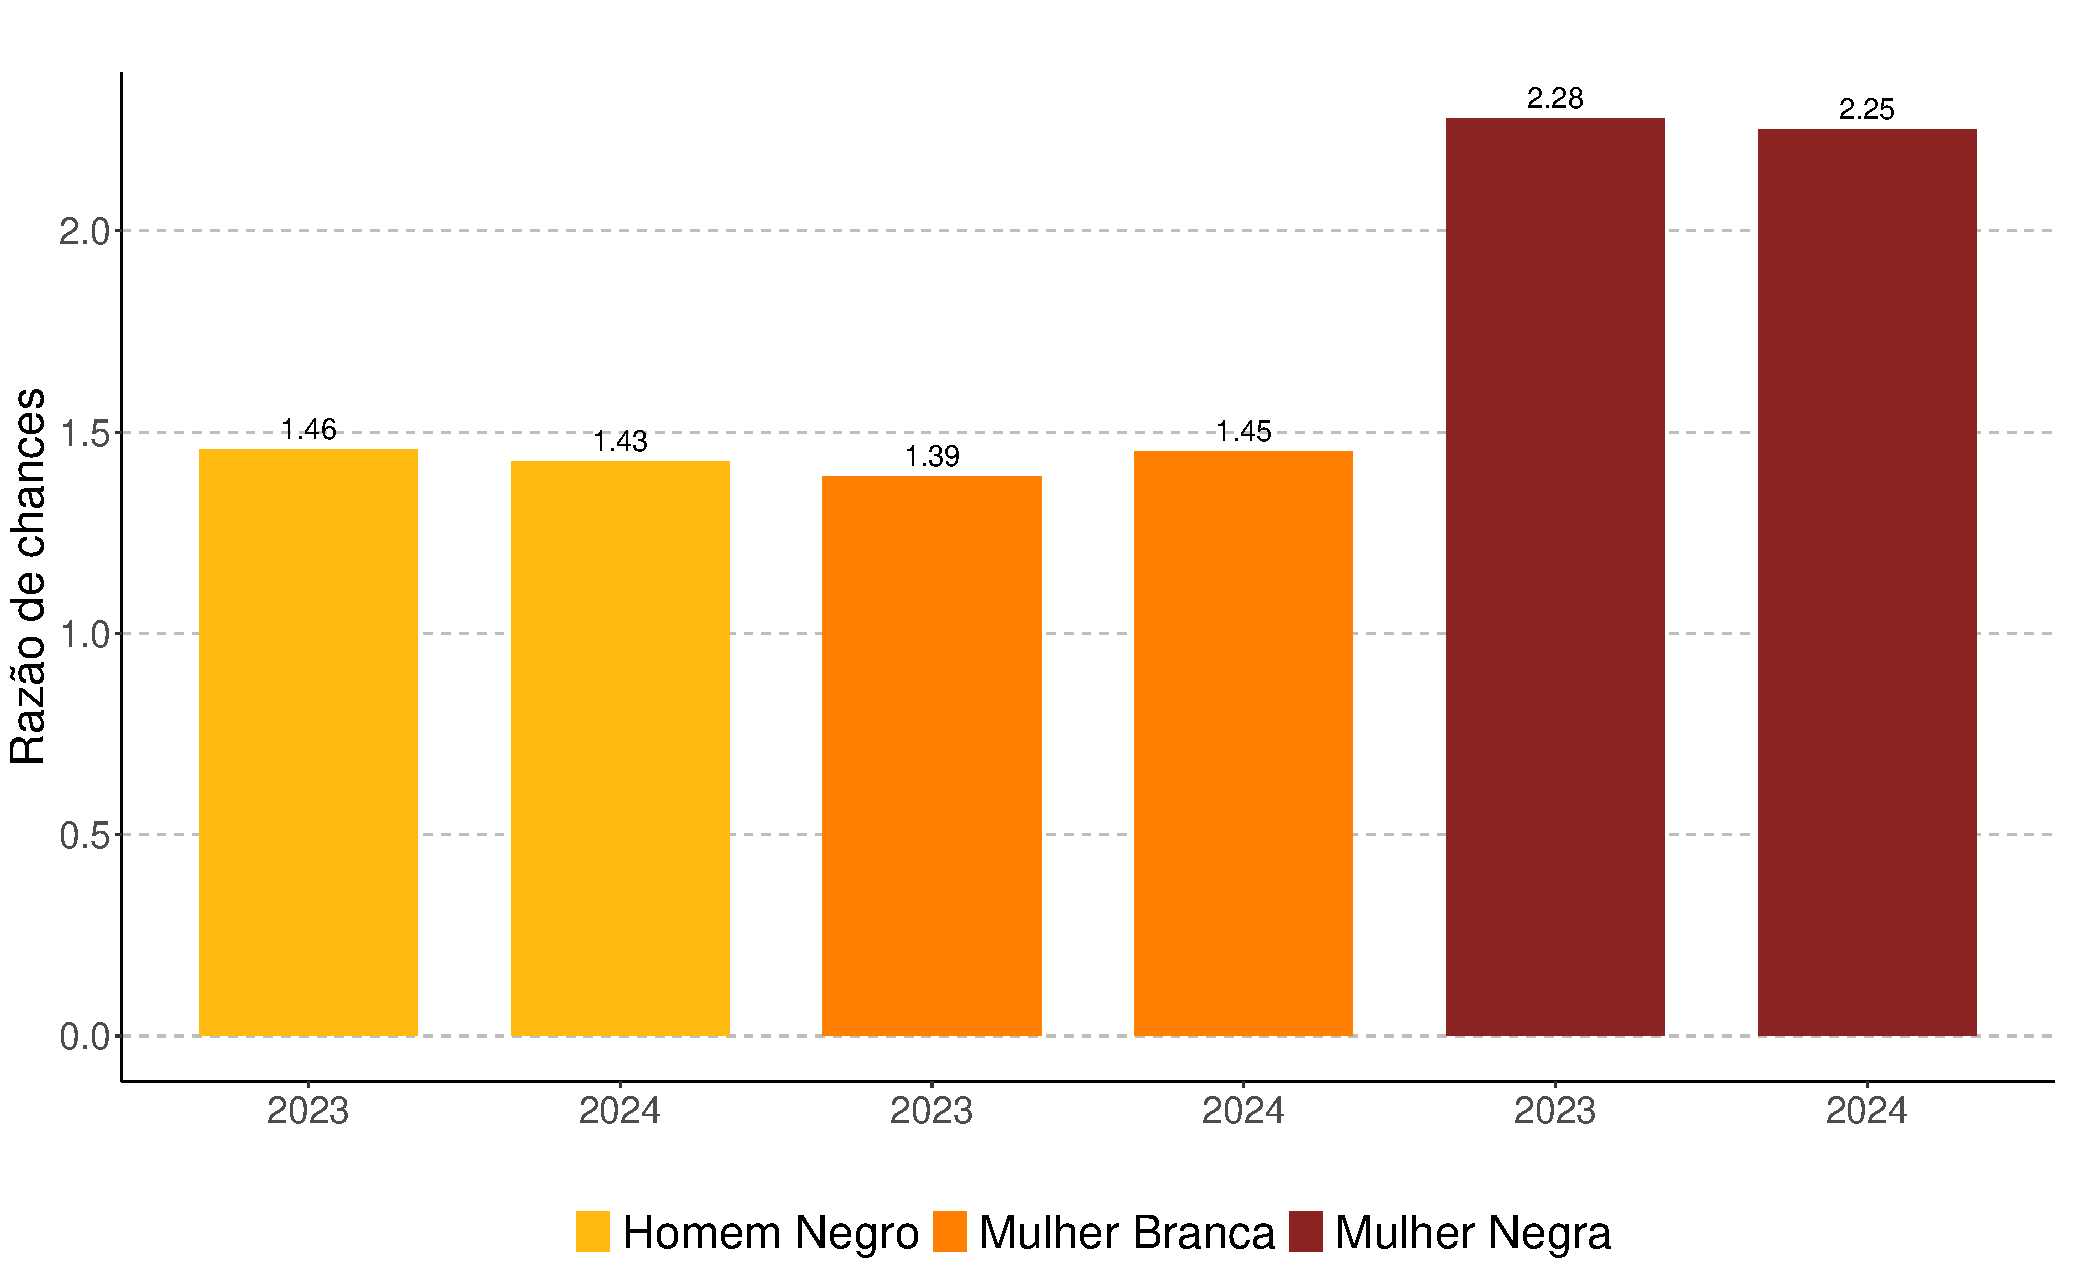
\includegraphics[width = 0.75\textwidth]{figures_output/frac_unemp.pdf}
		\end{figure}
		\end{frame}
	
	\begin{frame}{Taxa de Desemprego}
		\begin{figure}
			\centering
			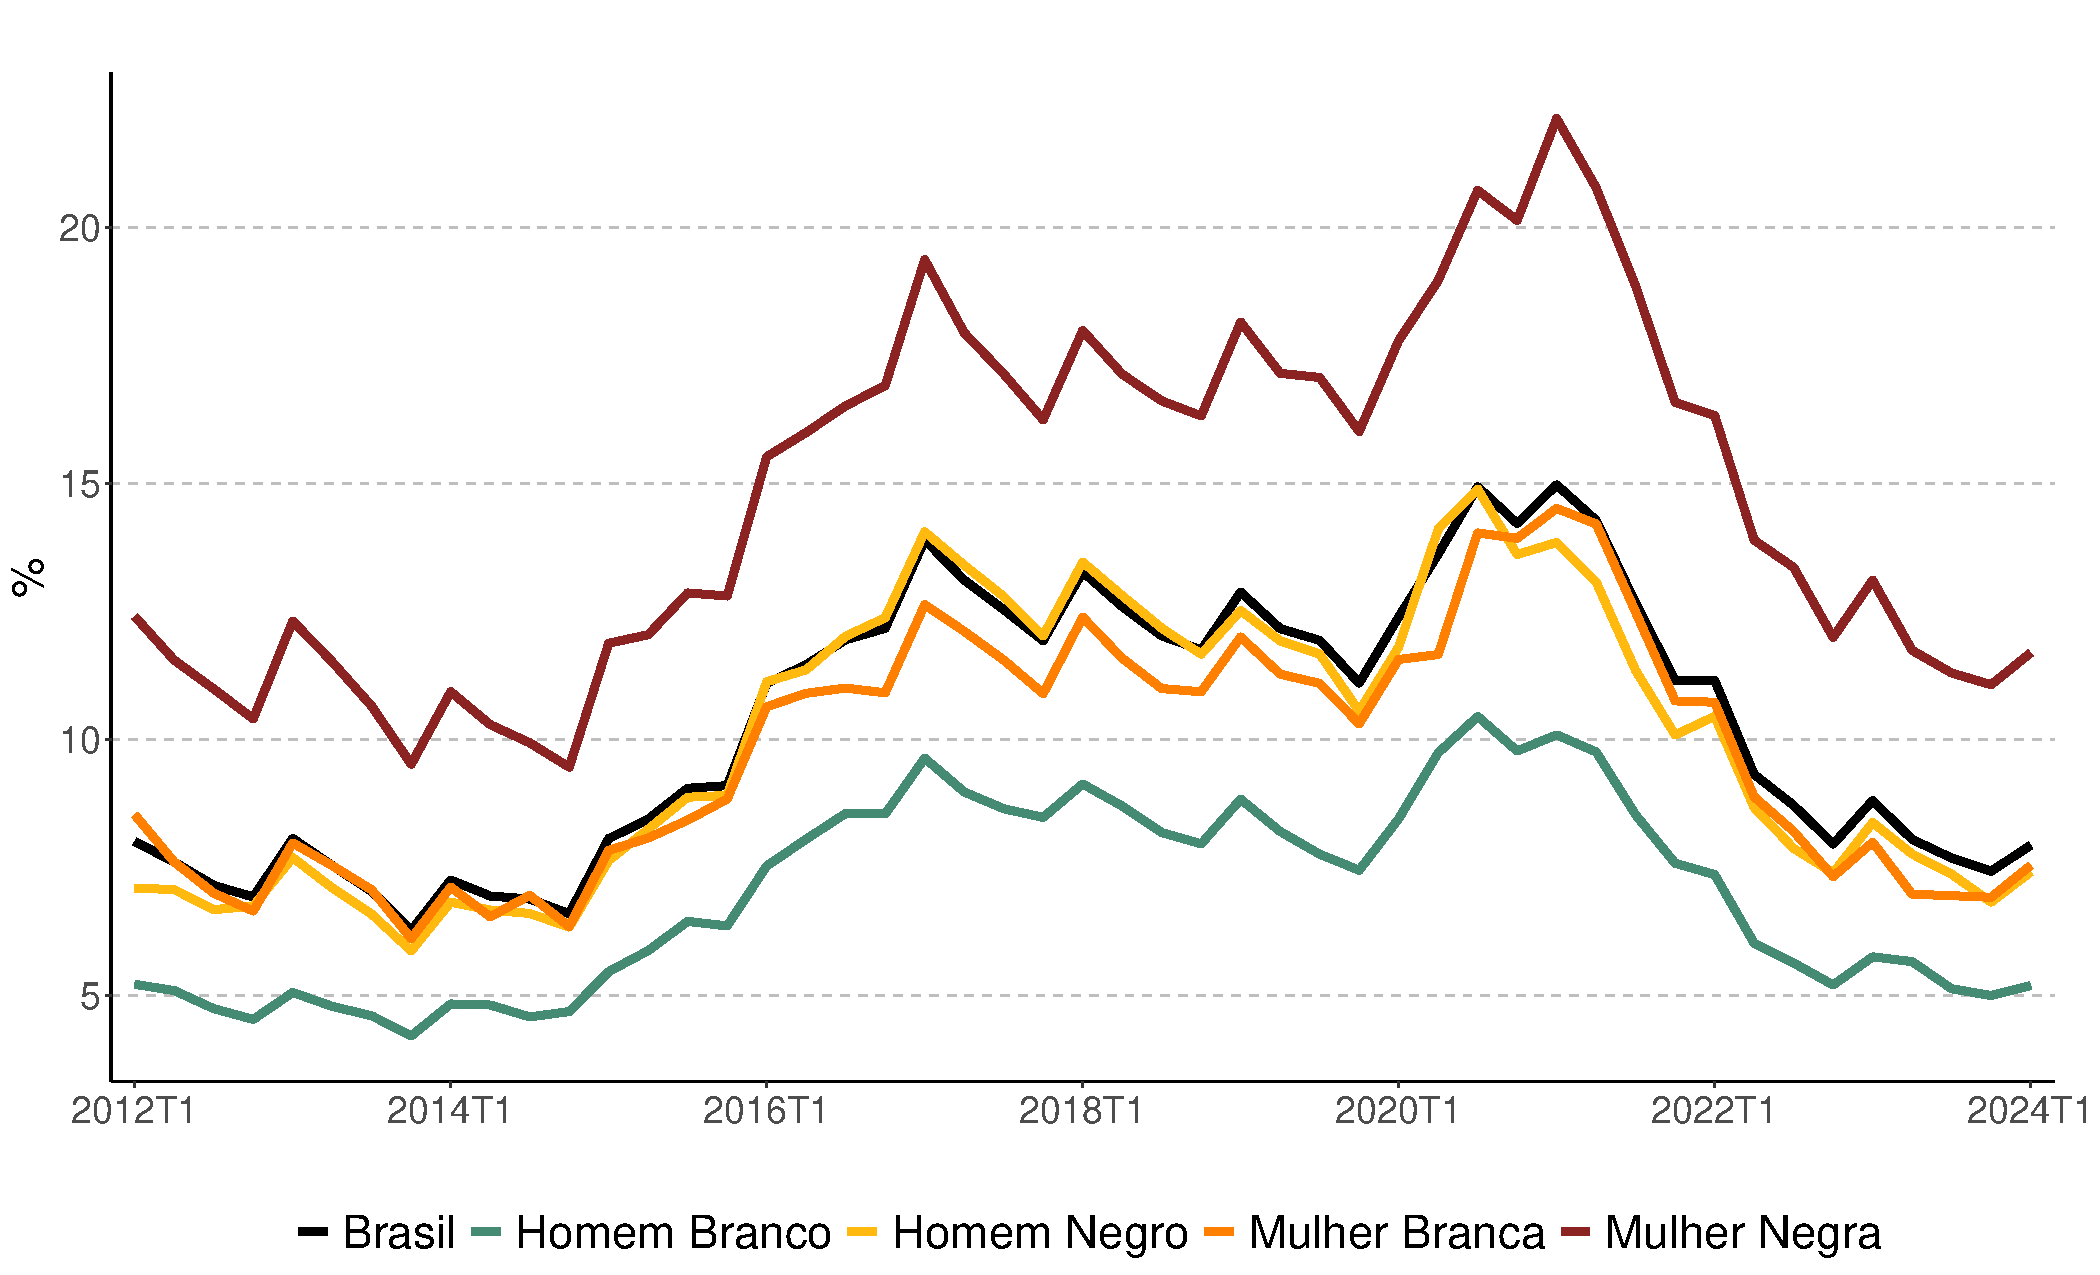
\includegraphics[width = 0.75\textwidth]{figures_output/unemp_br_gen_raca.pdf}
		\end{figure}
	\end{frame}			
	
		\begin{frame}{Desigualdade na PEA}
		\begin{figure}
			\centering
			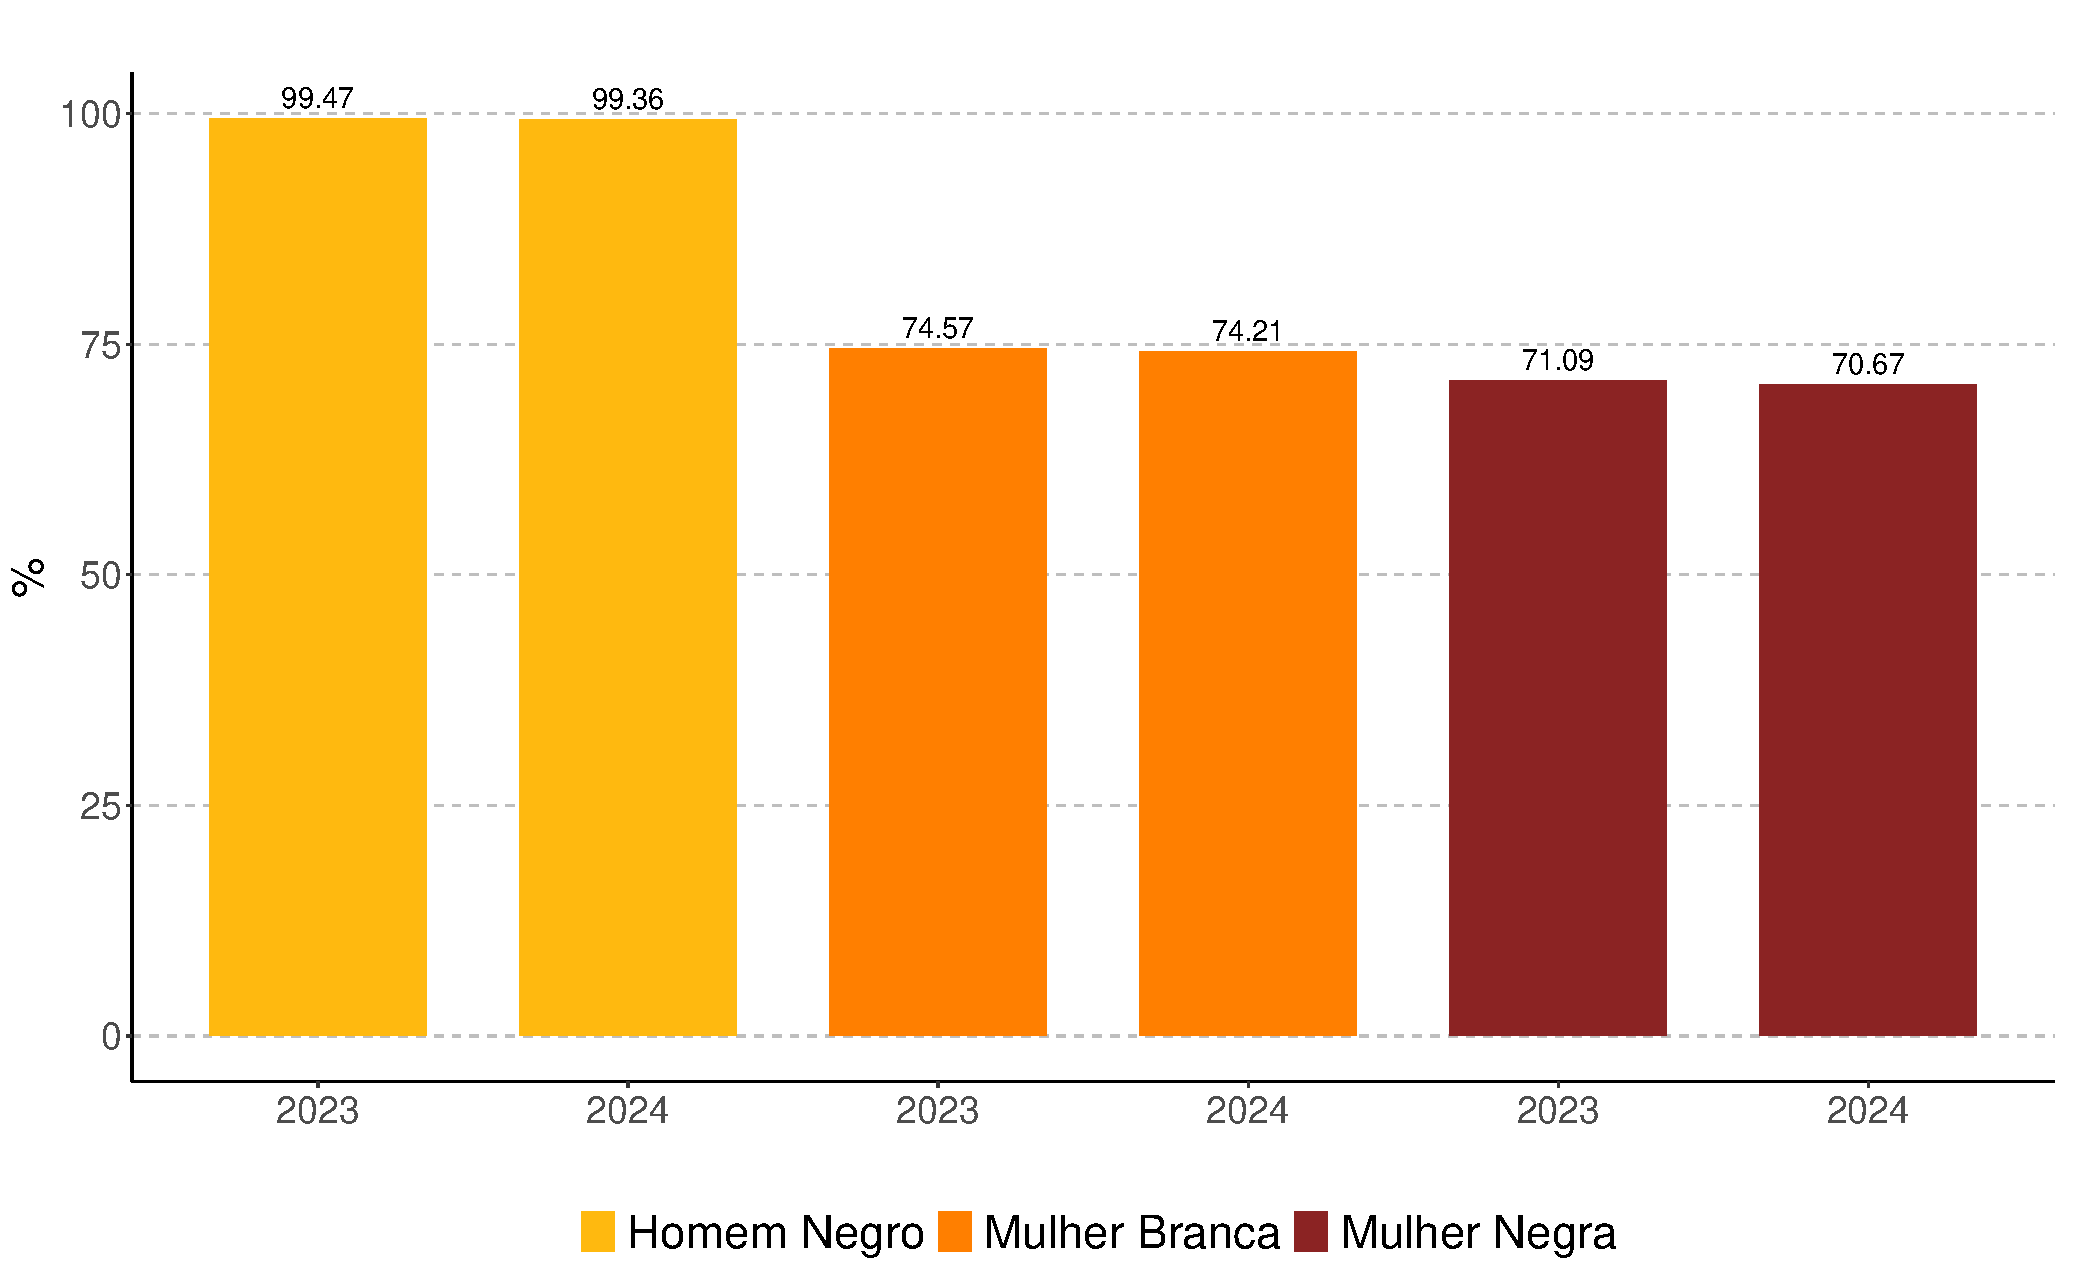
\includegraphics[width = 0.75\textwidth]{figures_output/frac_pea.pdf}
		\end{figure}
	\end{frame}	

	\begin{frame}{PEA Recente}
	\begin{figure}
		\centering
		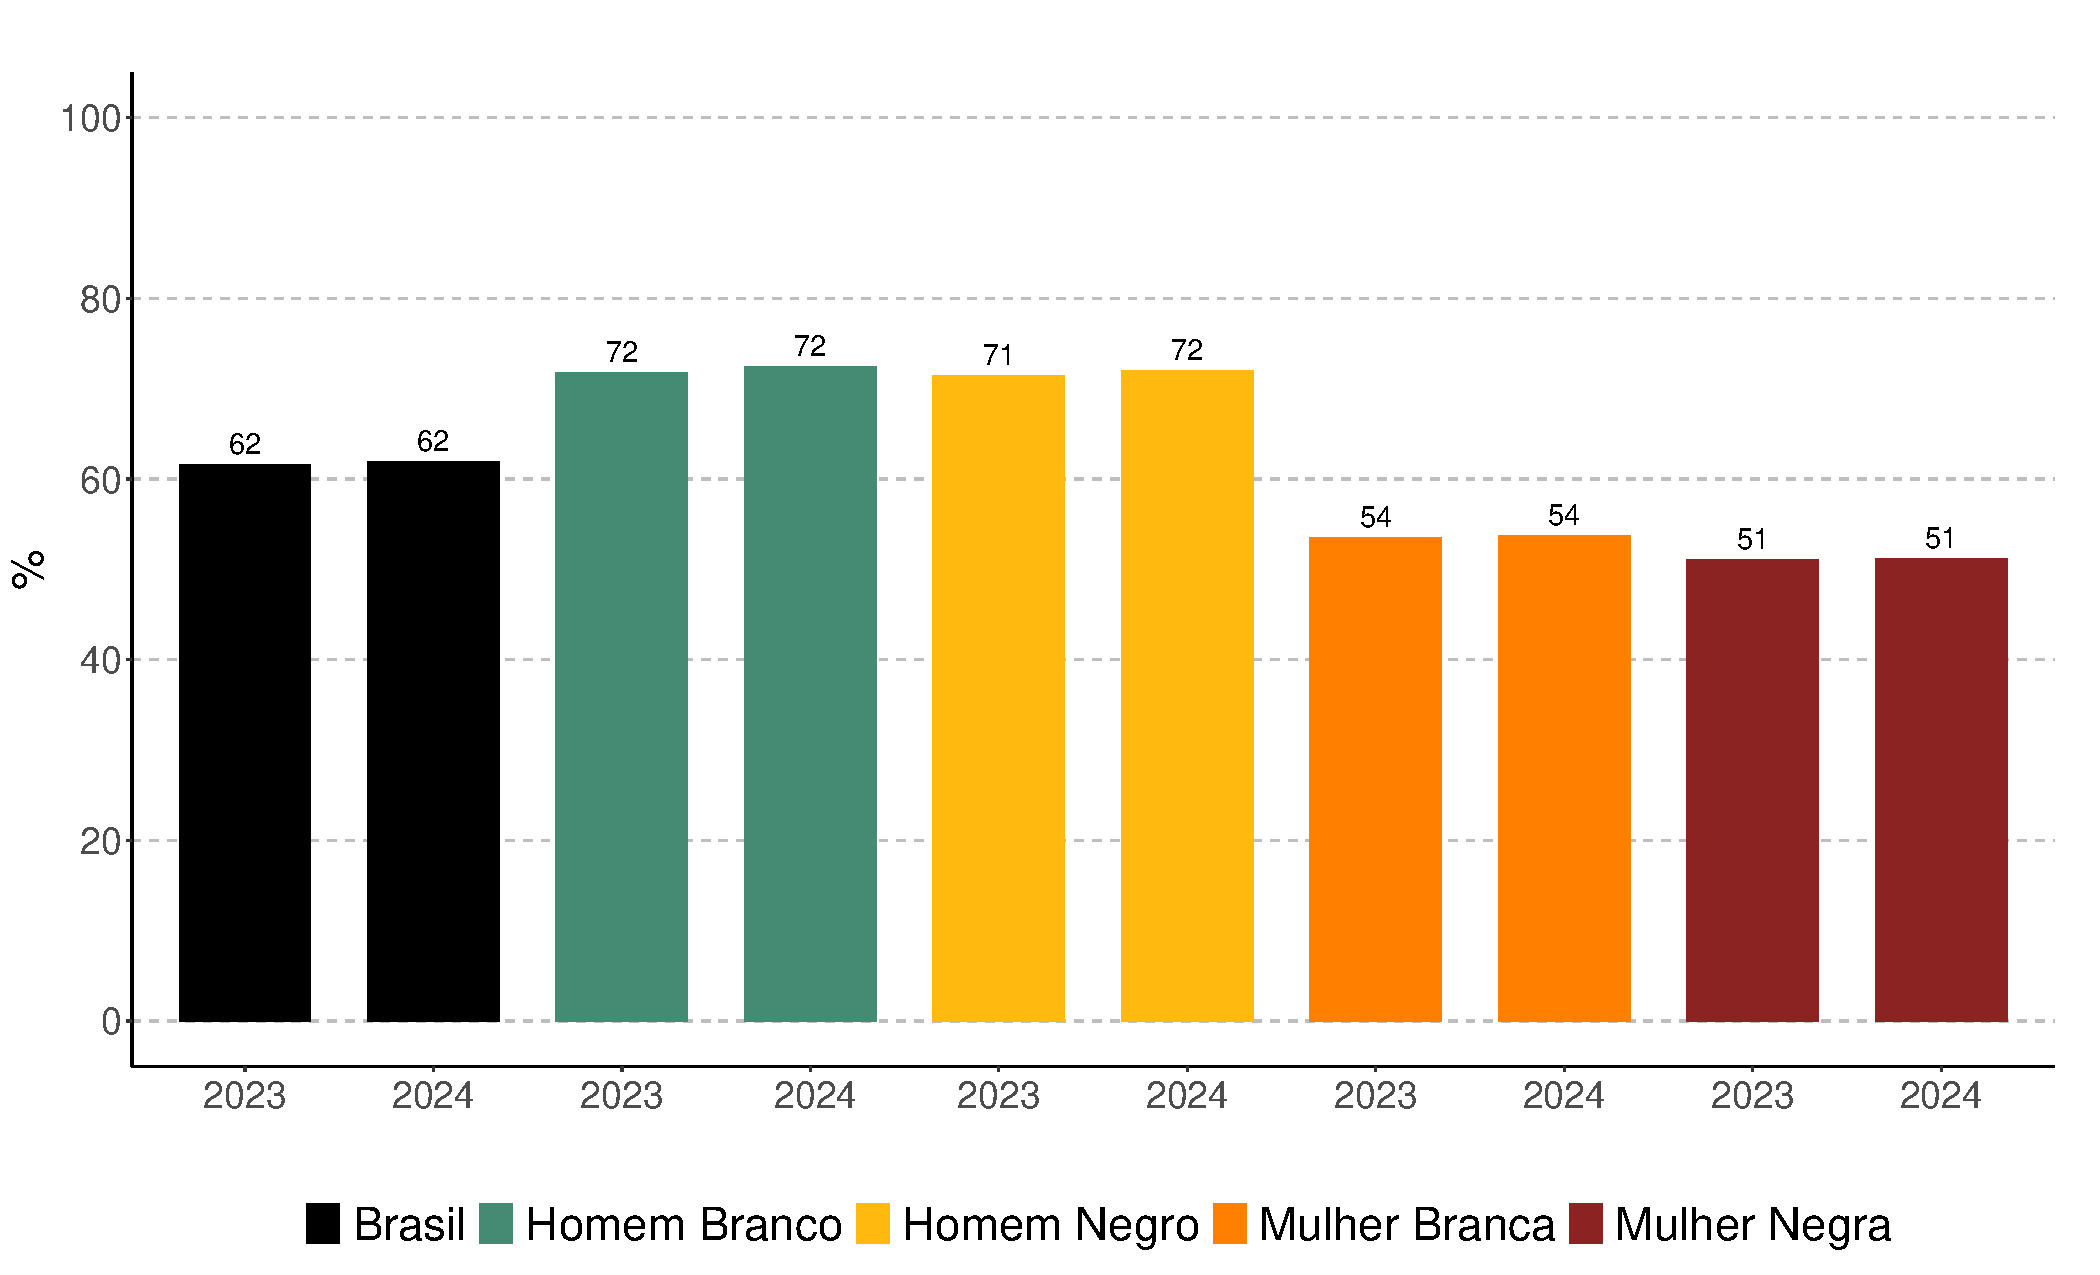
\includegraphics[width = 0.75\textwidth]{figures_output/pea.pdf}
	\end{figure}
	\end{frame}	

	\begin{frame}{PEA}
	\begin{figure}
		\centering
		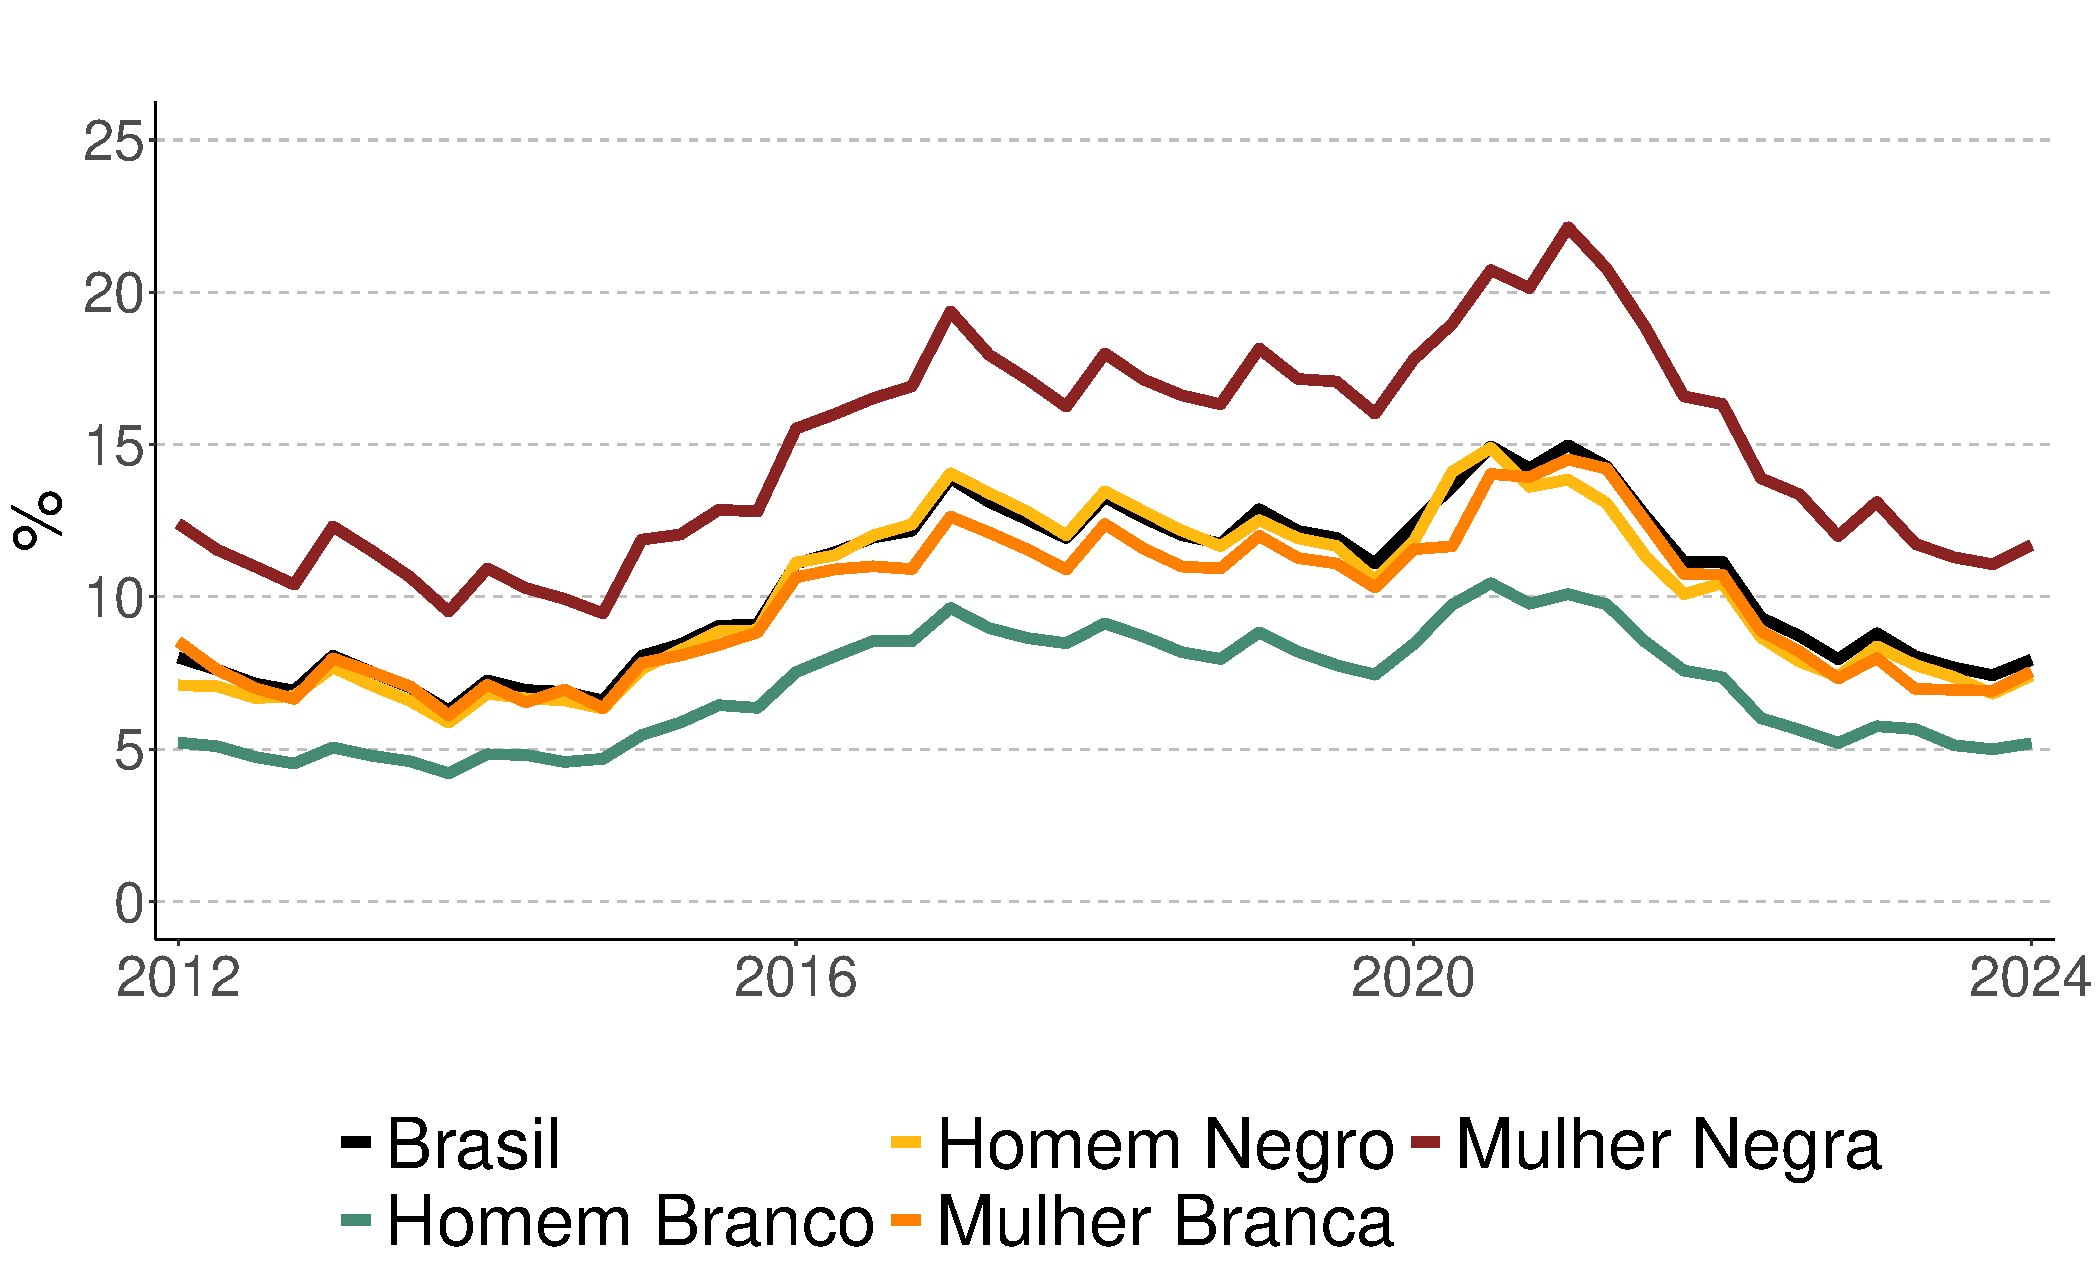
\includegraphics[width = 0.75\textwidth]{figures_output/pea_br_gen_raca.pdf}
	\end{figure}
	\end{frame}	
	
	
	\begin{frame}{Gini}
		\begin{figure}
			\centering
			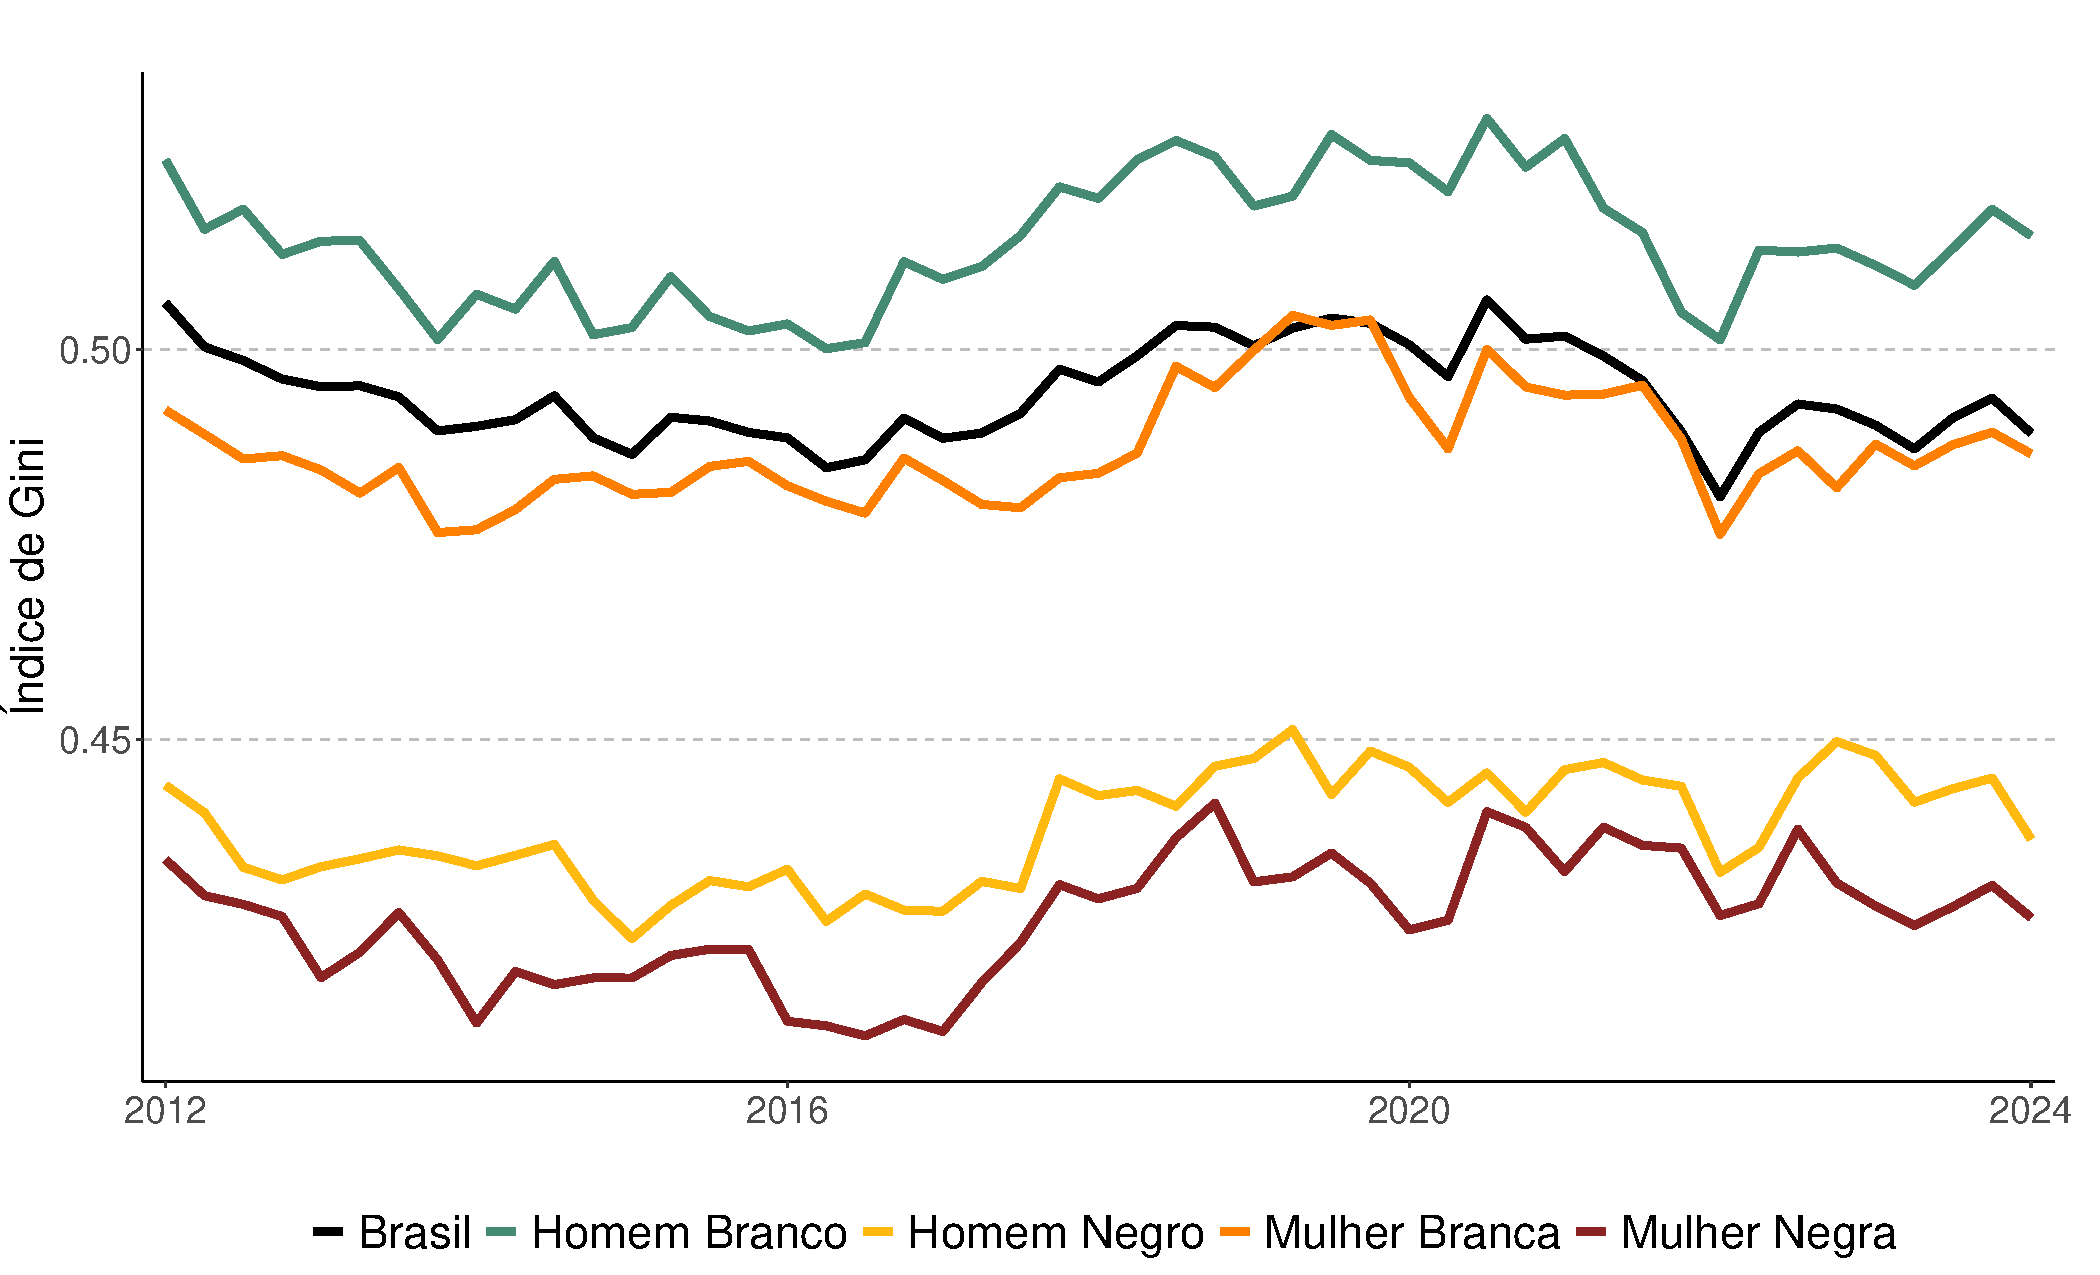
\includegraphics[width = 0.75\textwidth]{figures_output/gini_br_gen_raca.pdf}
		\end{figure}
	\end{frame}
	
	\begin{frame}{A Base e o Topo da Distribuição}
	\begin{figure}
		\centering
		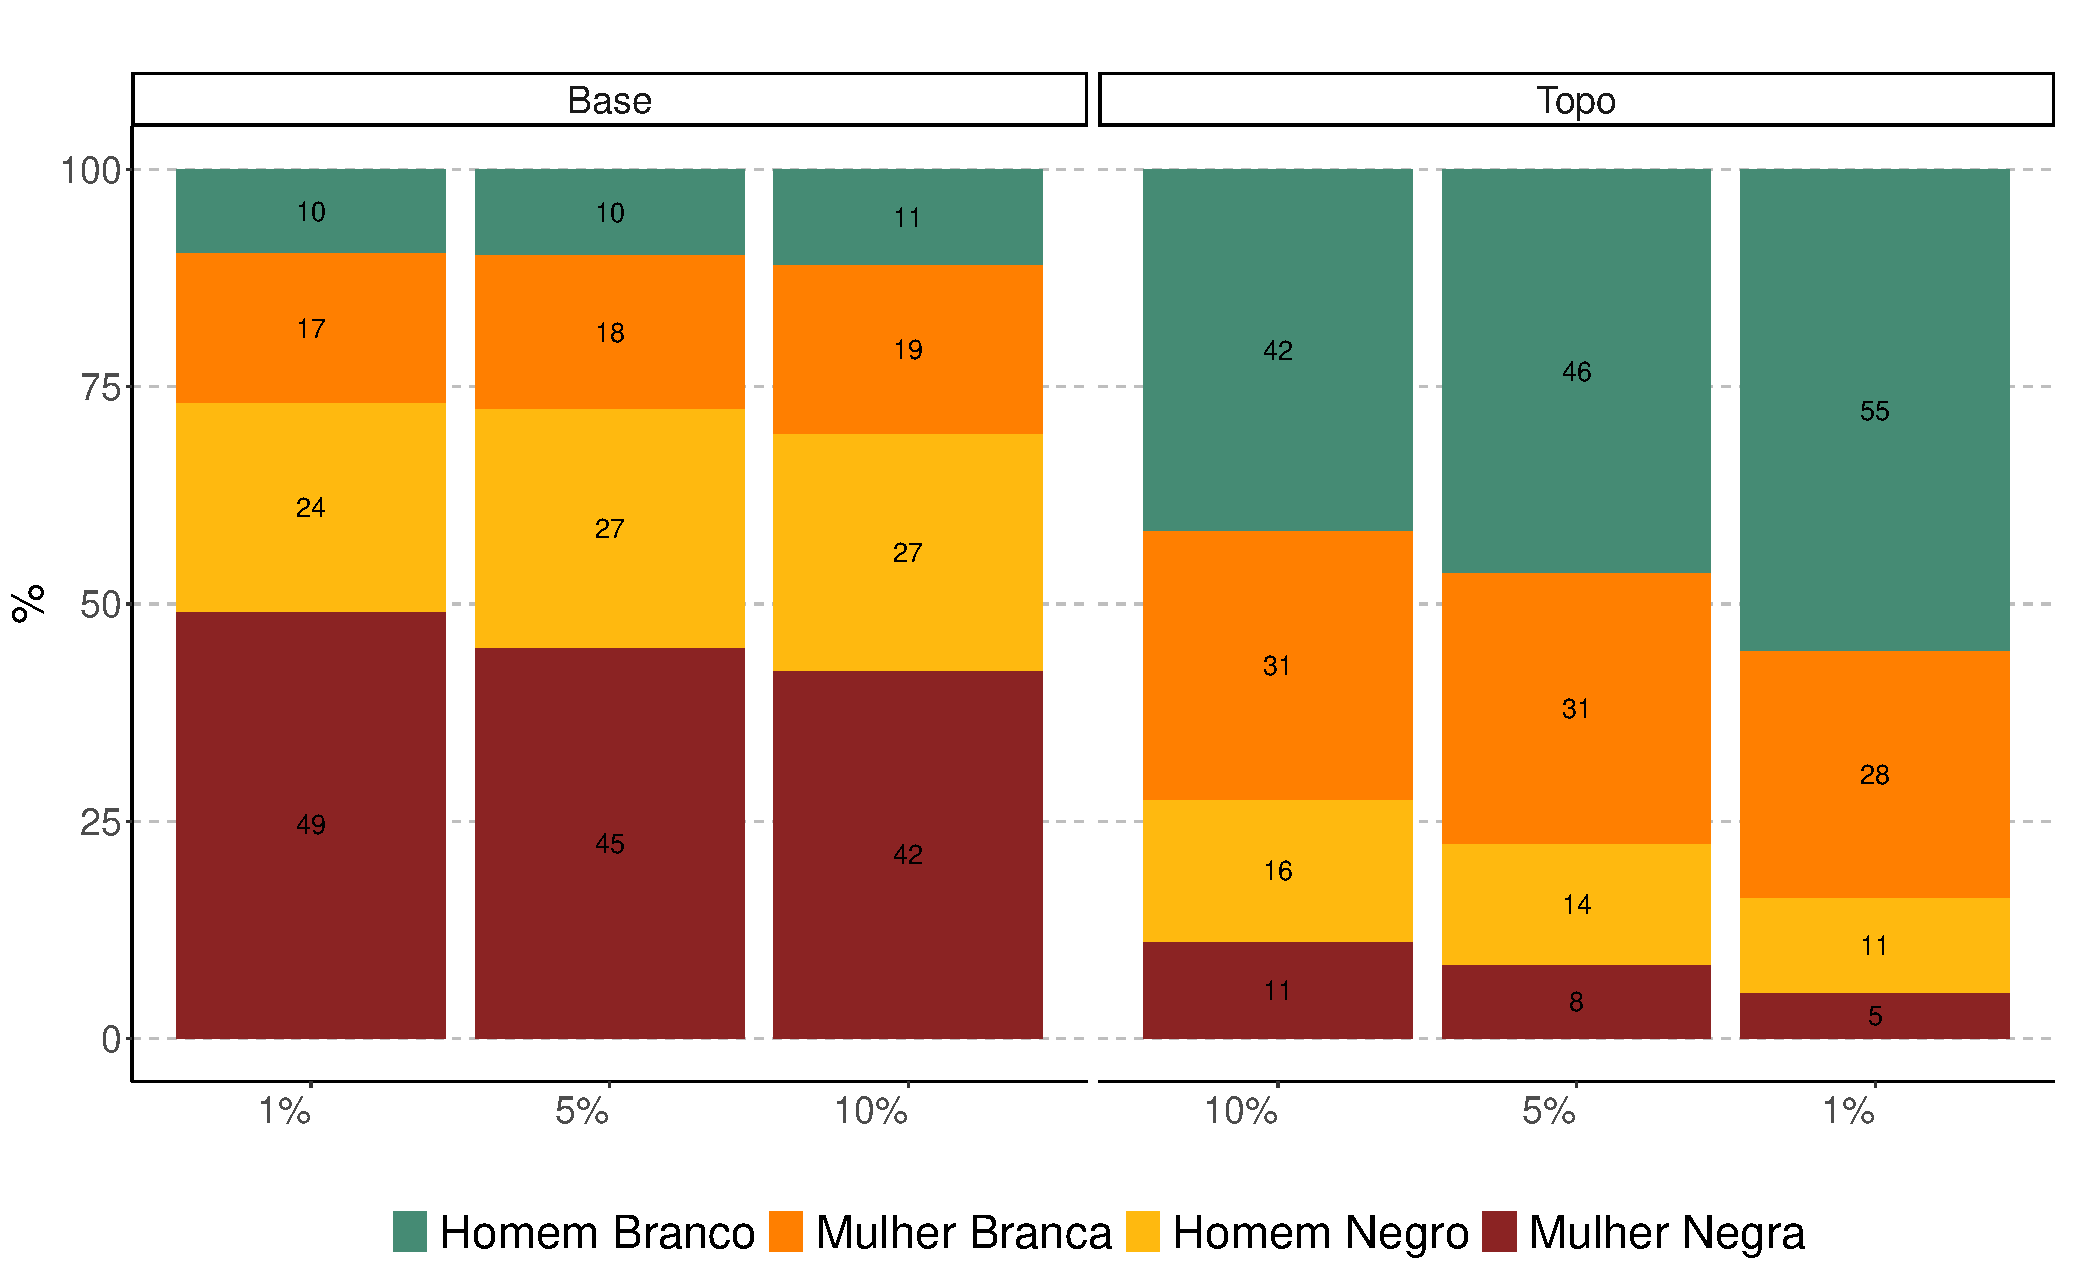
\includegraphics[width = 0.75\textwidth]{figures_output/top_bottom.pdf}
	\end{figure}
	\end{frame}
	
	\begin{frame}{Massa Salarial Recente}
	\begin{figure}
		\centering
		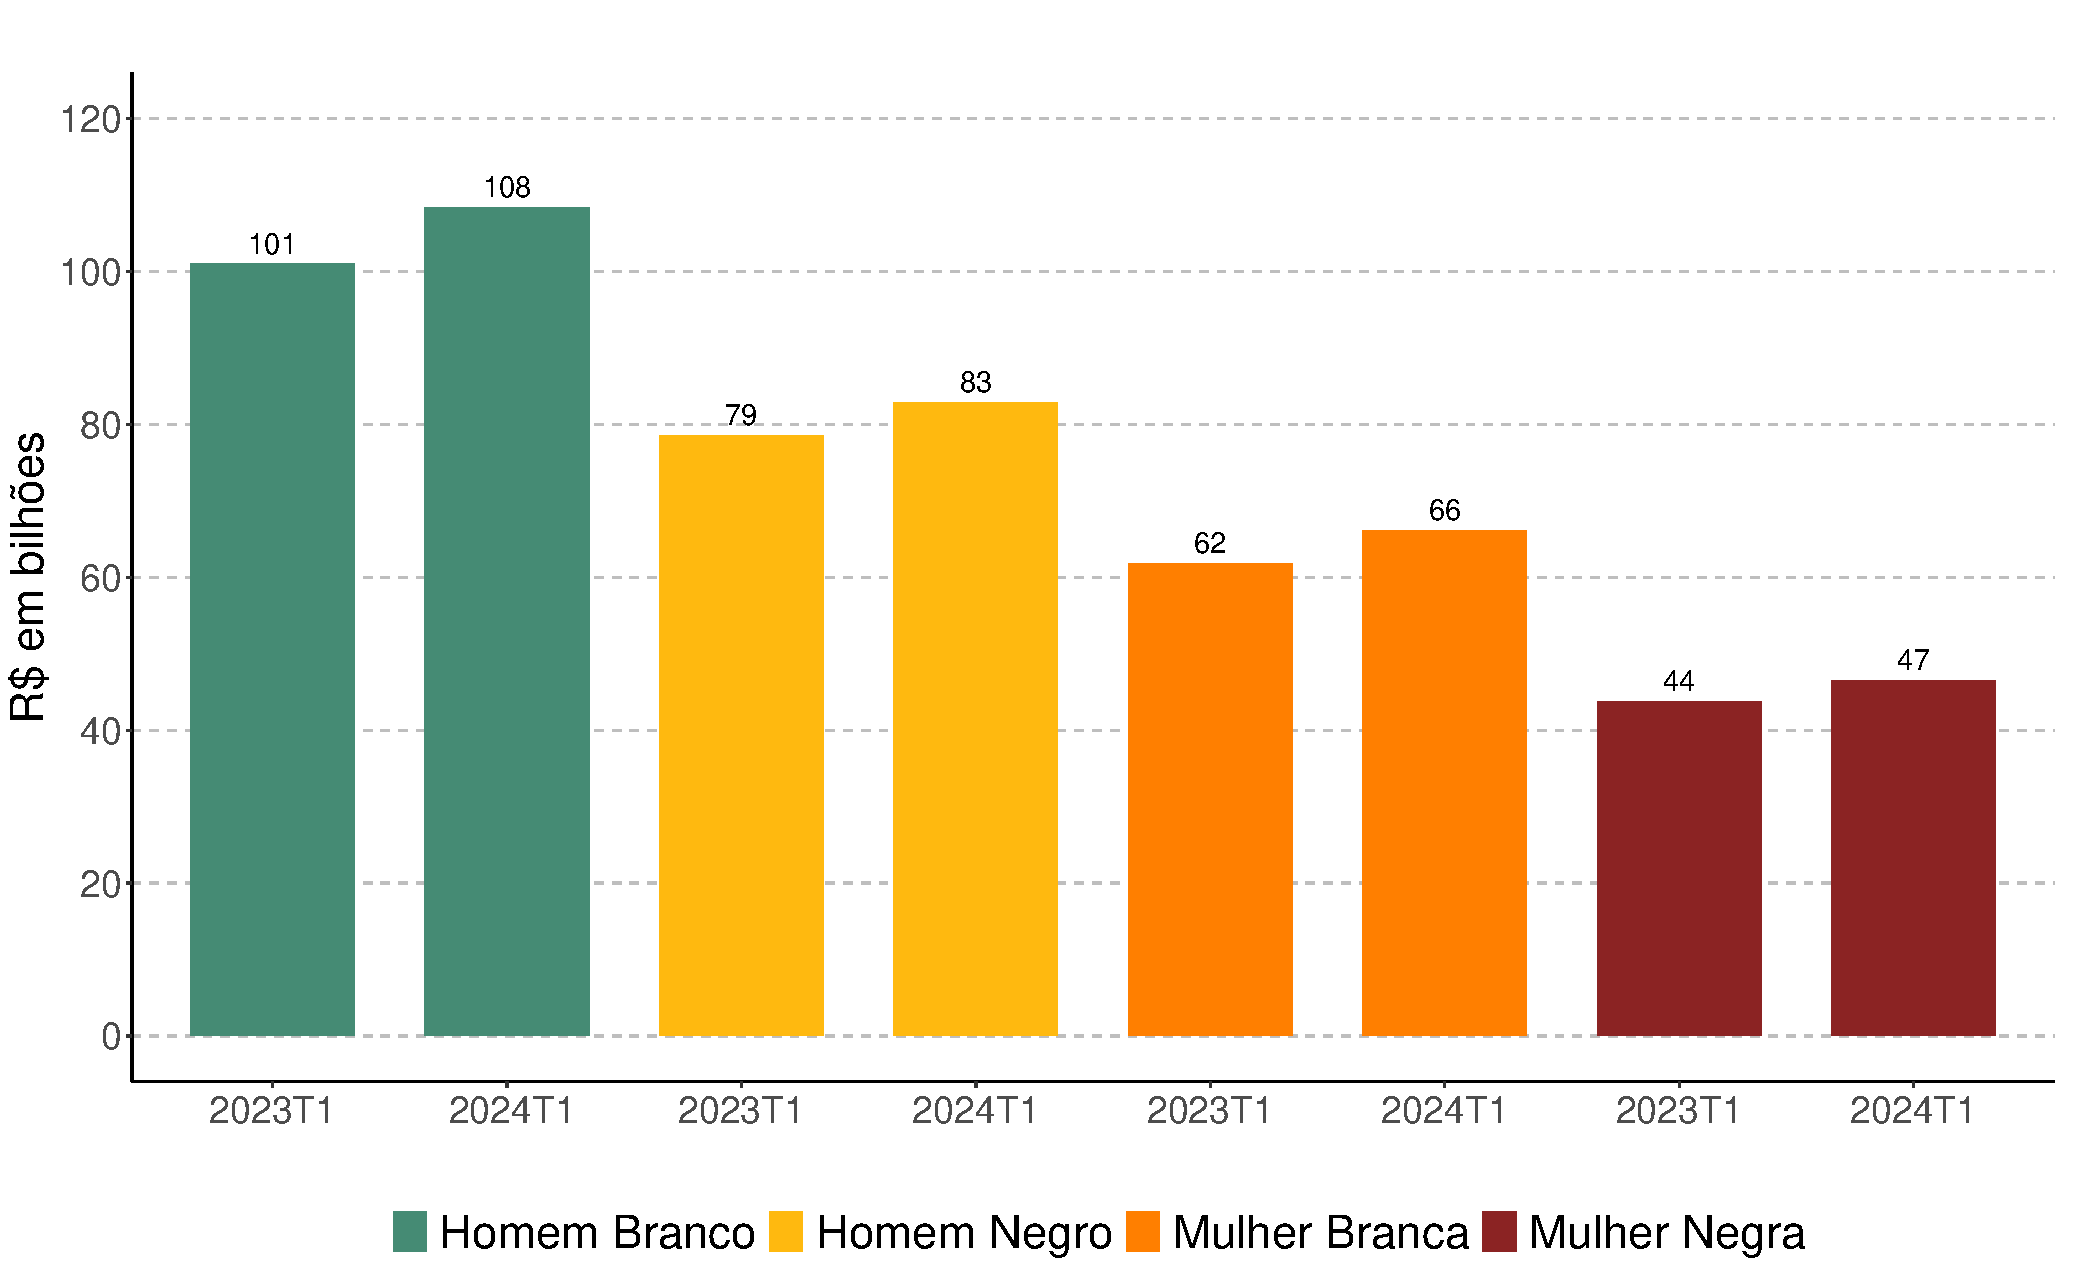
\includegraphics[width = 0.75\textwidth]{figures_output/massa_habitual.pdf}
	\end{figure}
	\end{frame}
	
	\begin{frame}{Massa Salarial Habitual}
		\begin{figure}
			\centering
			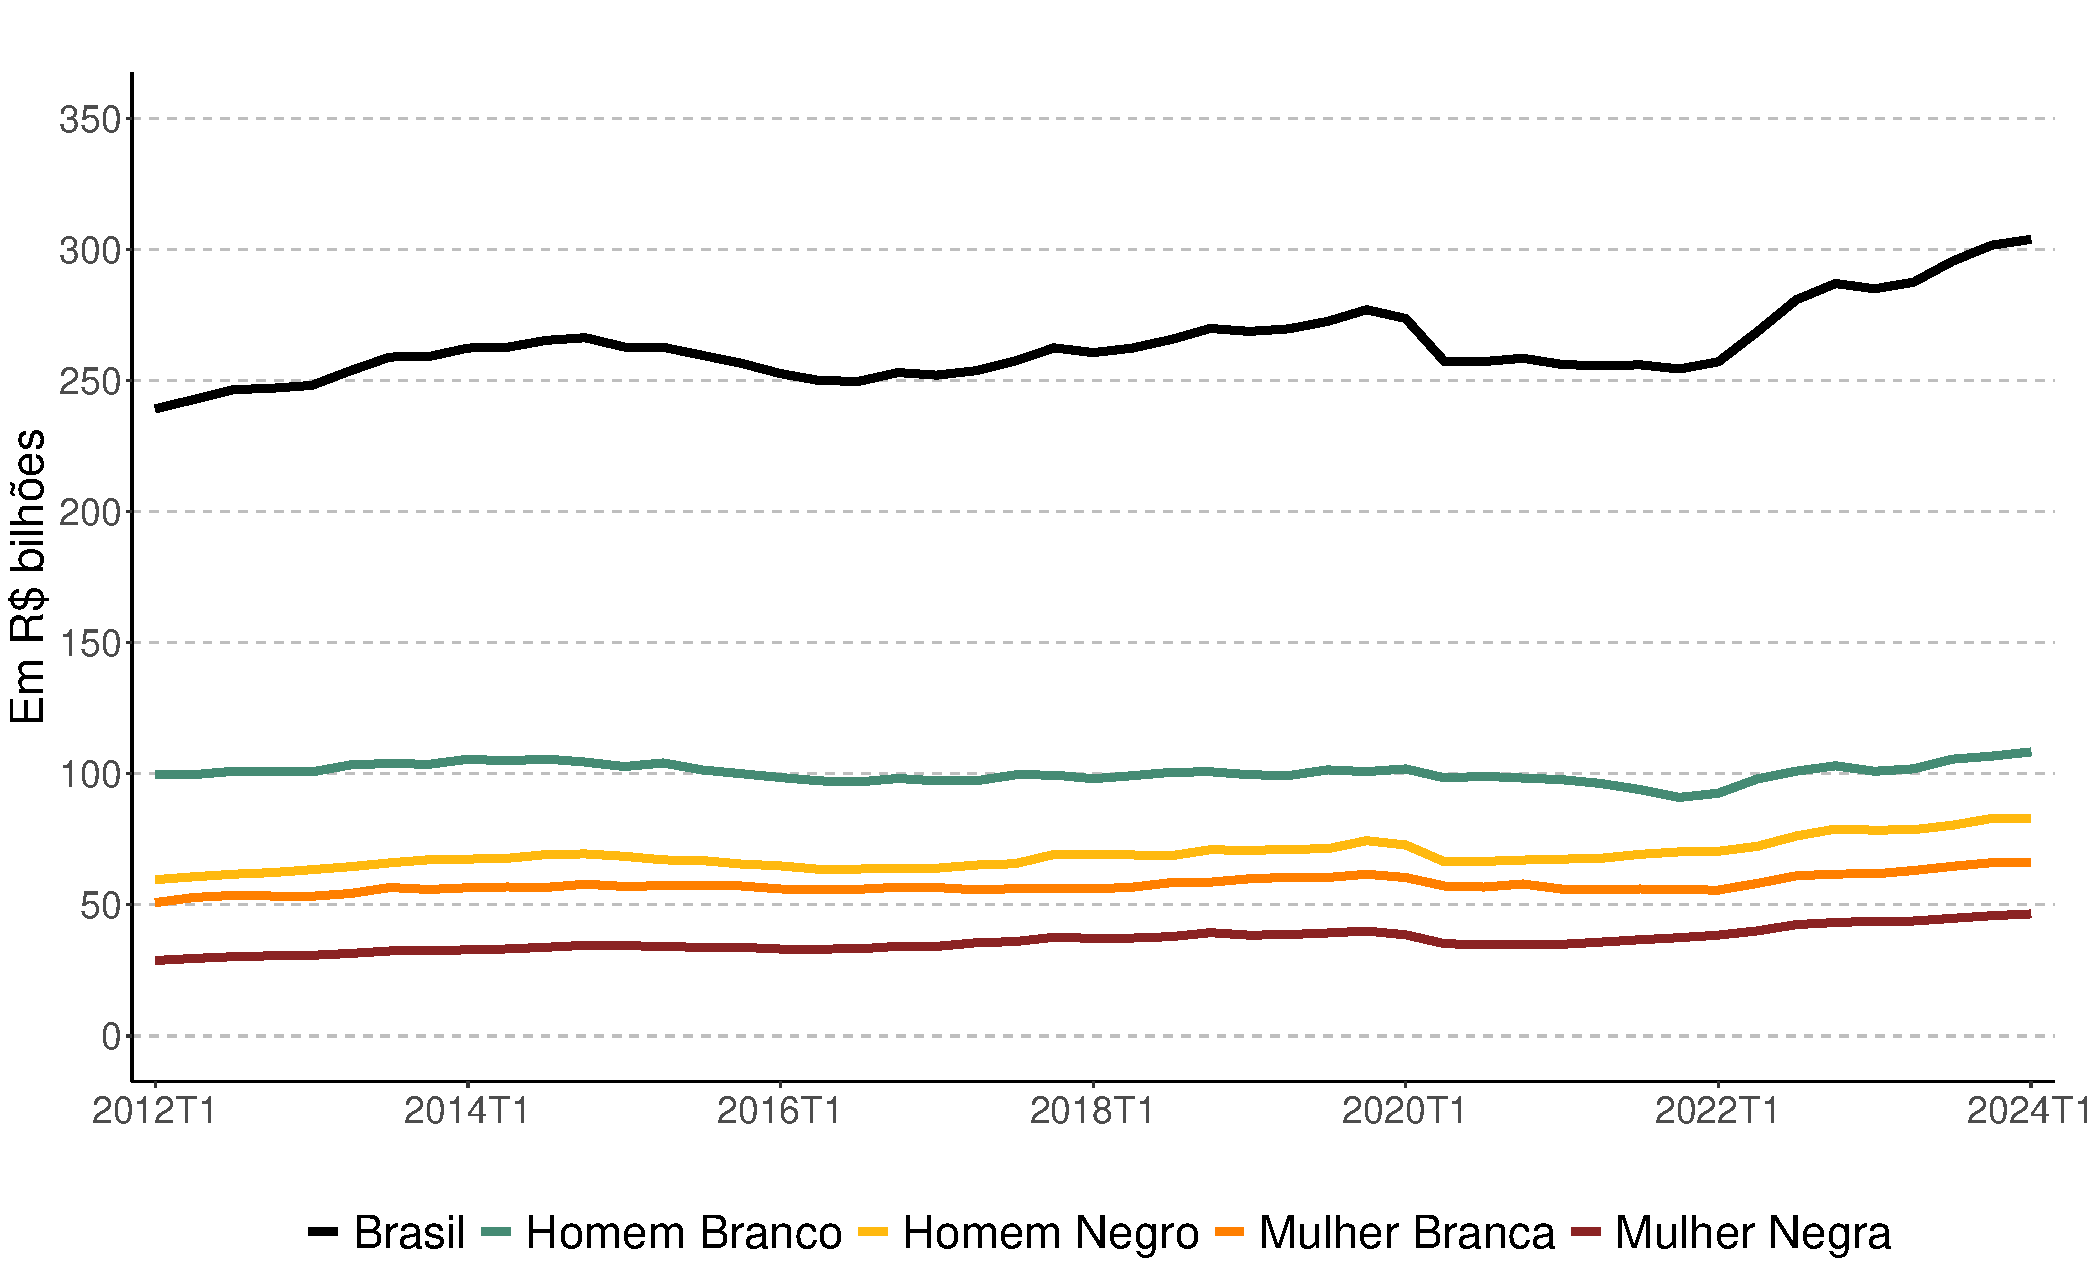
\includegraphics[width = 0.75\textwidth]{figures_output/massa_habitual_br_gen_raca.pdf}
		\end{figure}
	\end{frame}
	
	\begin{frame}{Desigualdade na Massa Salarial}
		\begin{figure}
			\centering
			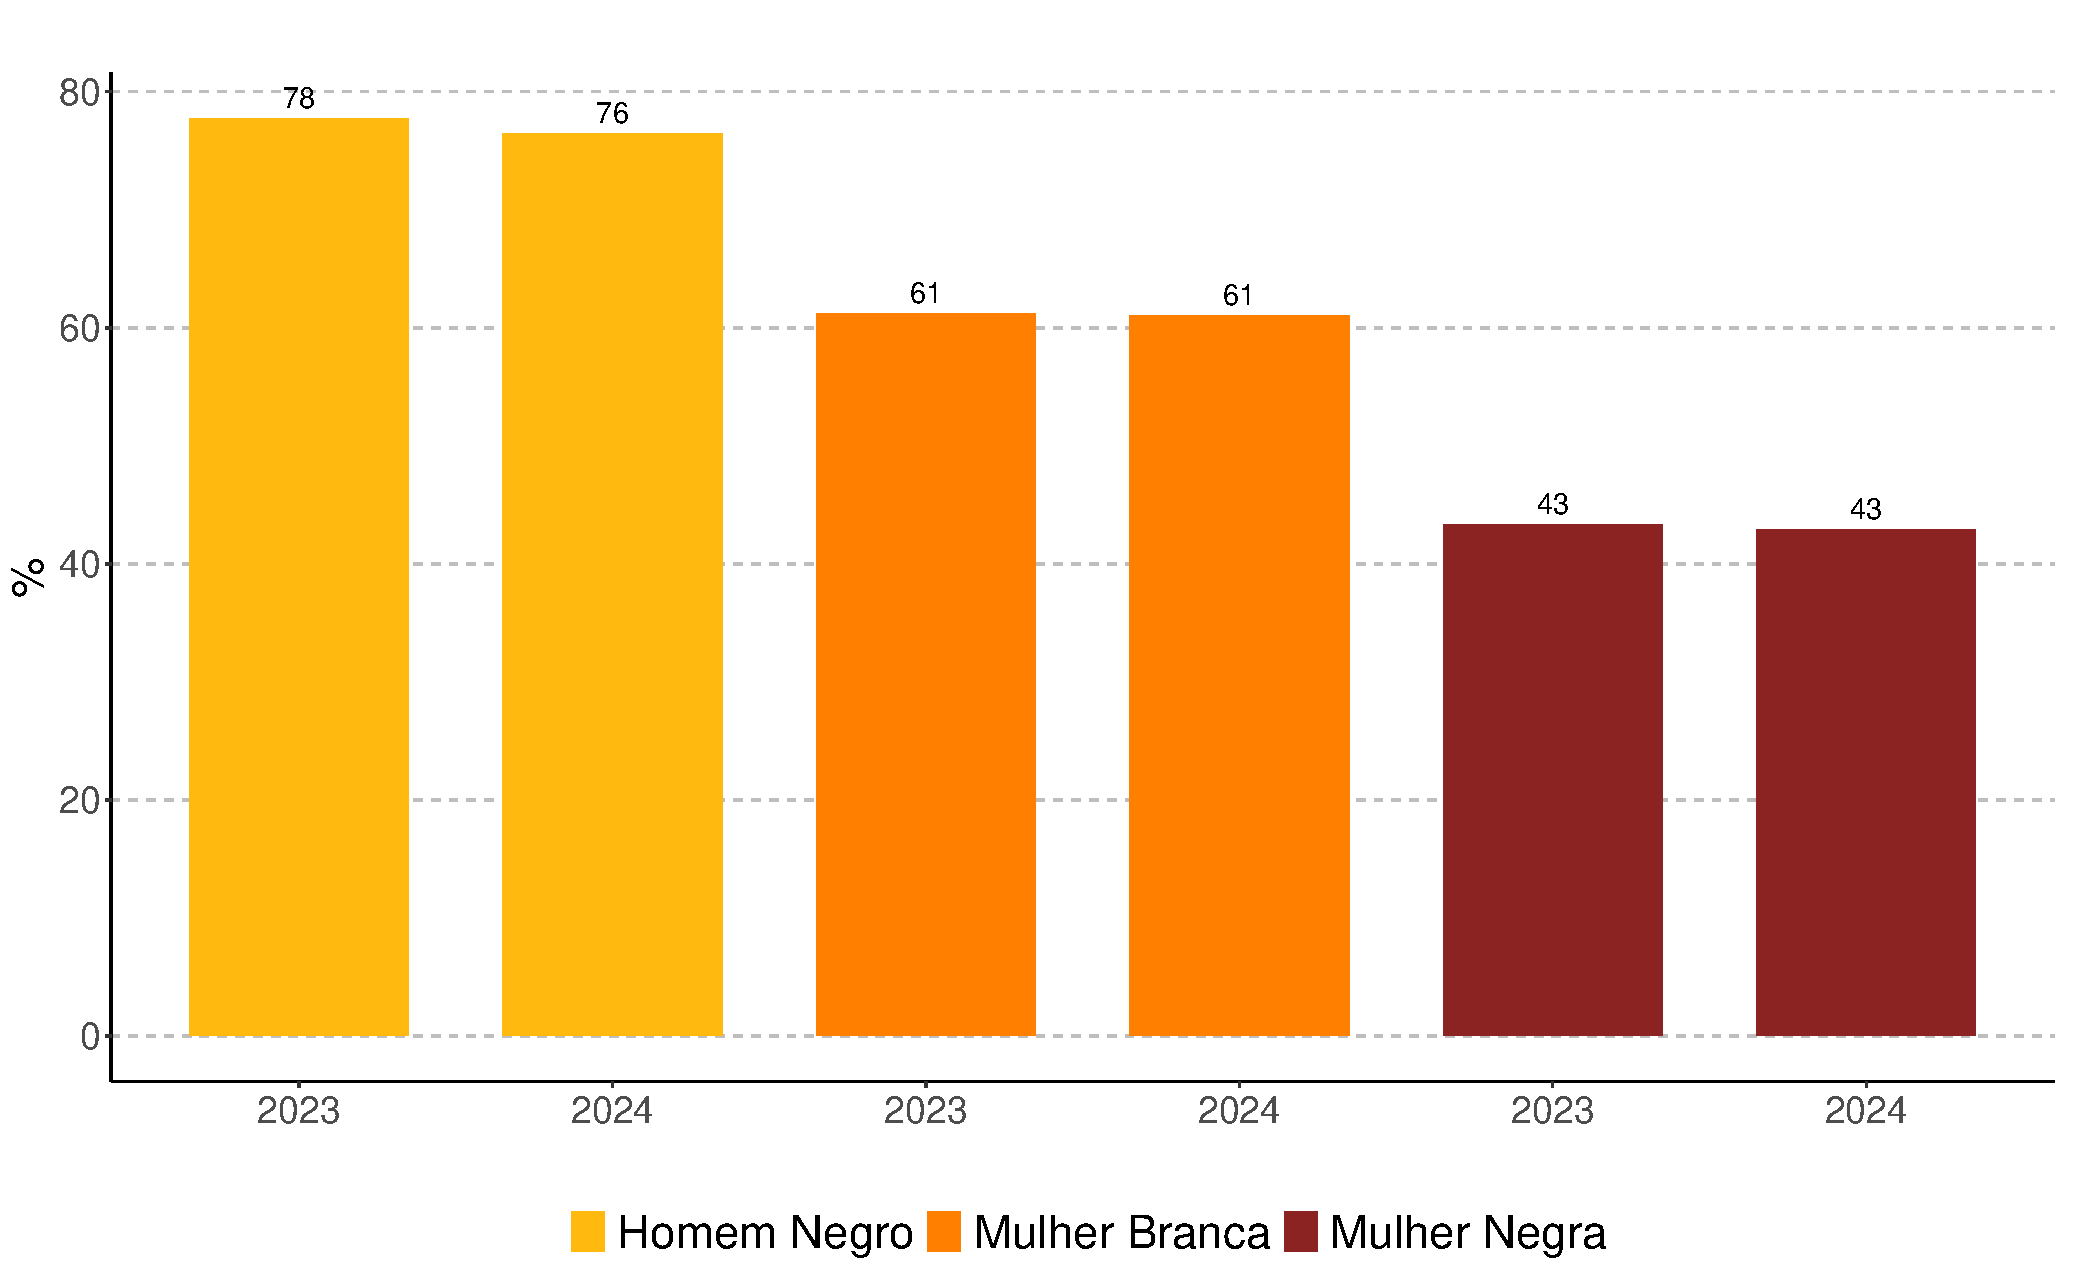
\includegraphics[width = 0.75\textwidth]{figures_output/frac_massa_habitual.pdf}
		\end{figure}
	\end{frame}		
	
\section{Estimando a Massa Salarial Perdida para Desigualdade}
	\begin{frame}{Massa Salarial Perdida}
	\begin{figure}
		\centering
		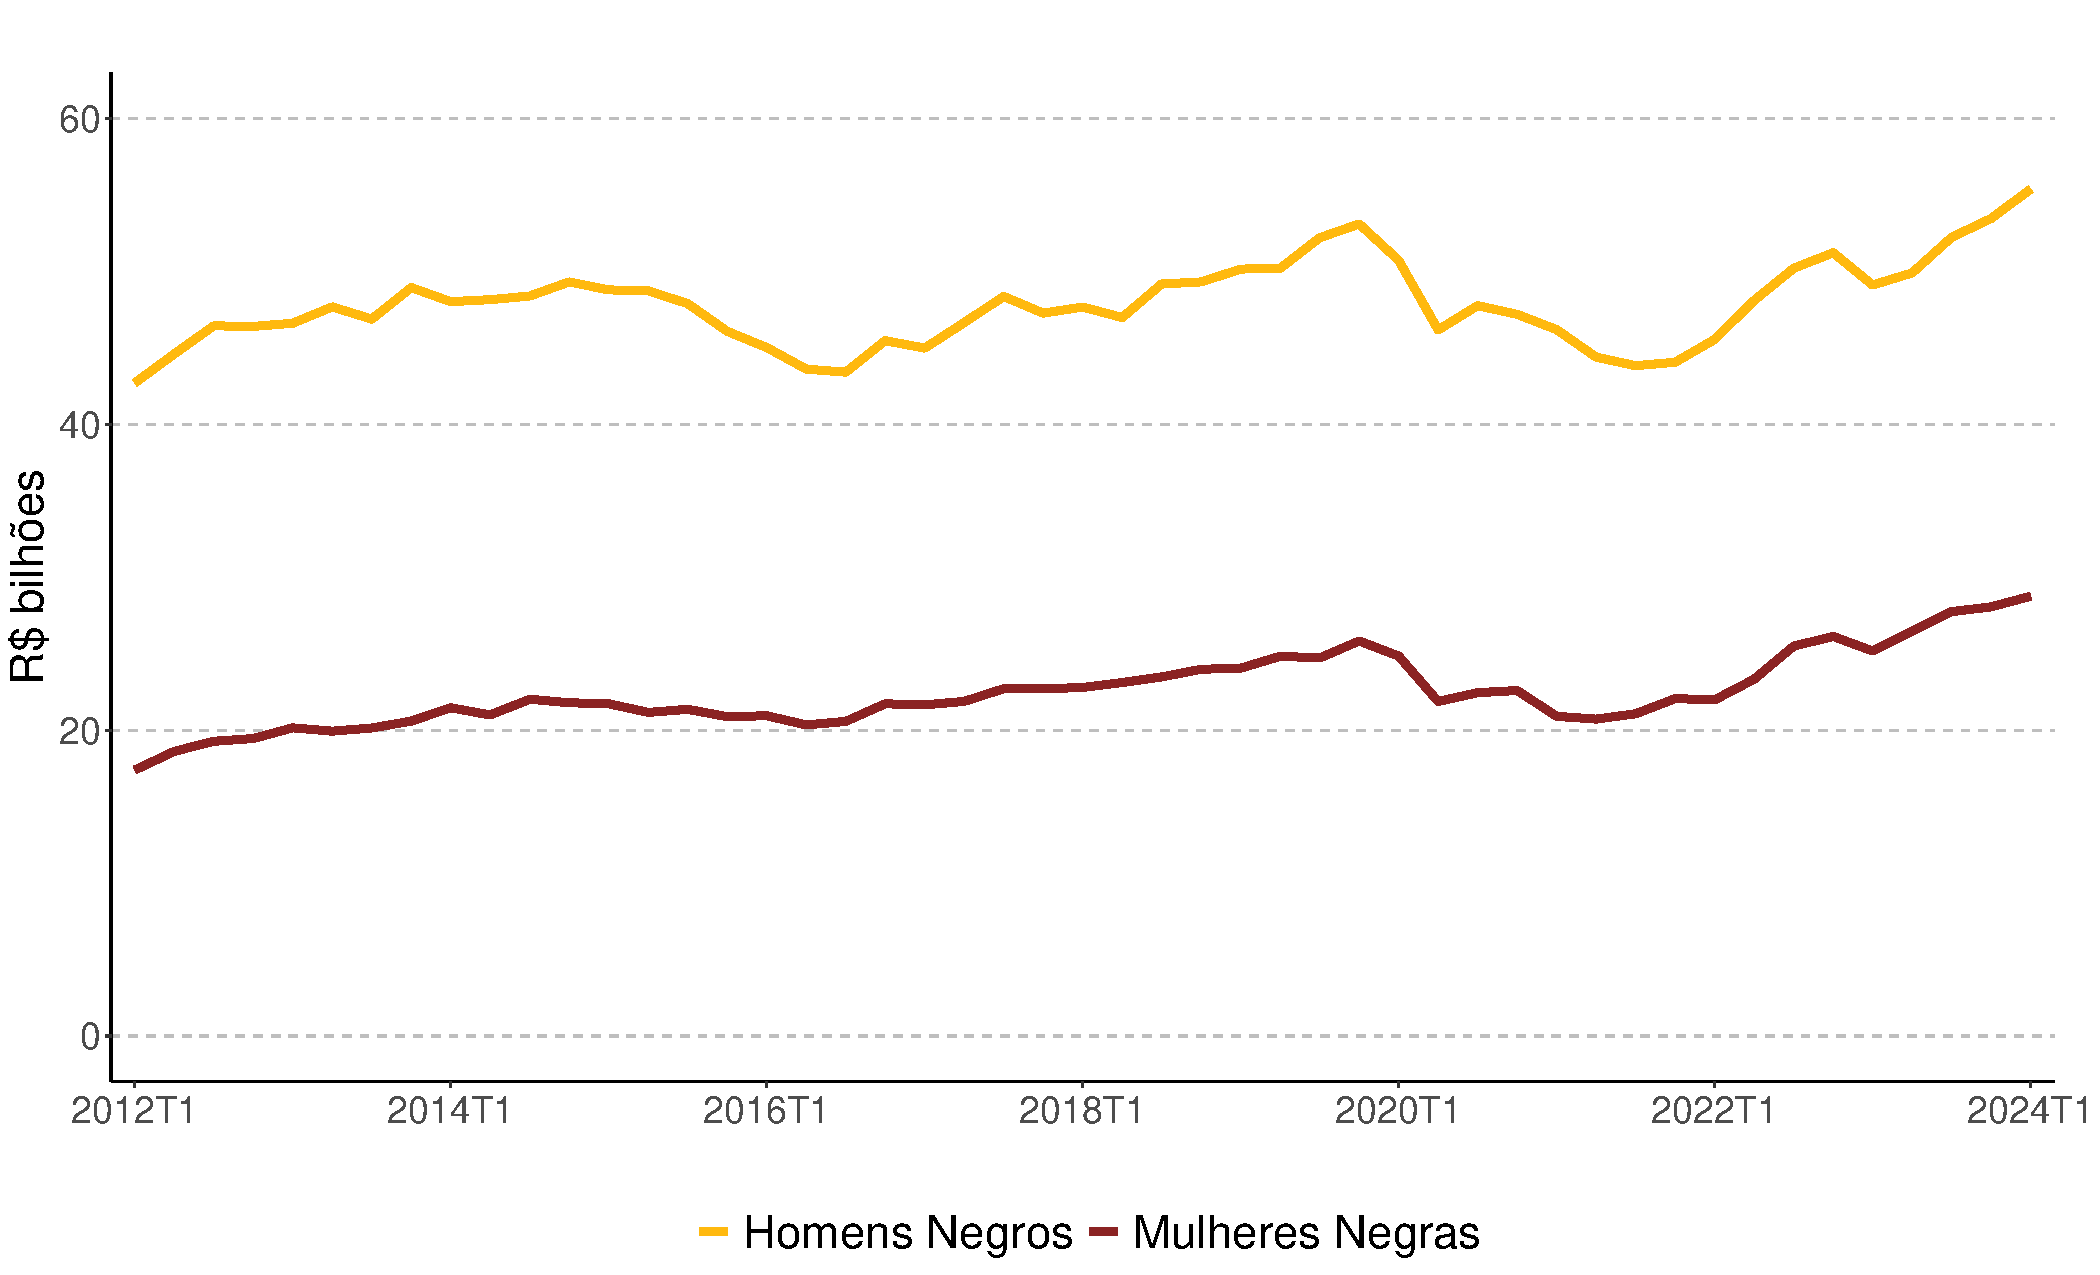
\includegraphics[width = 0.75\textwidth]{figures_output/perda_massa_salarial.pdf}
	\end{figure}
\end{frame}	

	\begin{frame}{Massa Salarial Perdida - Efeito Composição}
	\begin{figure}
		\centering
		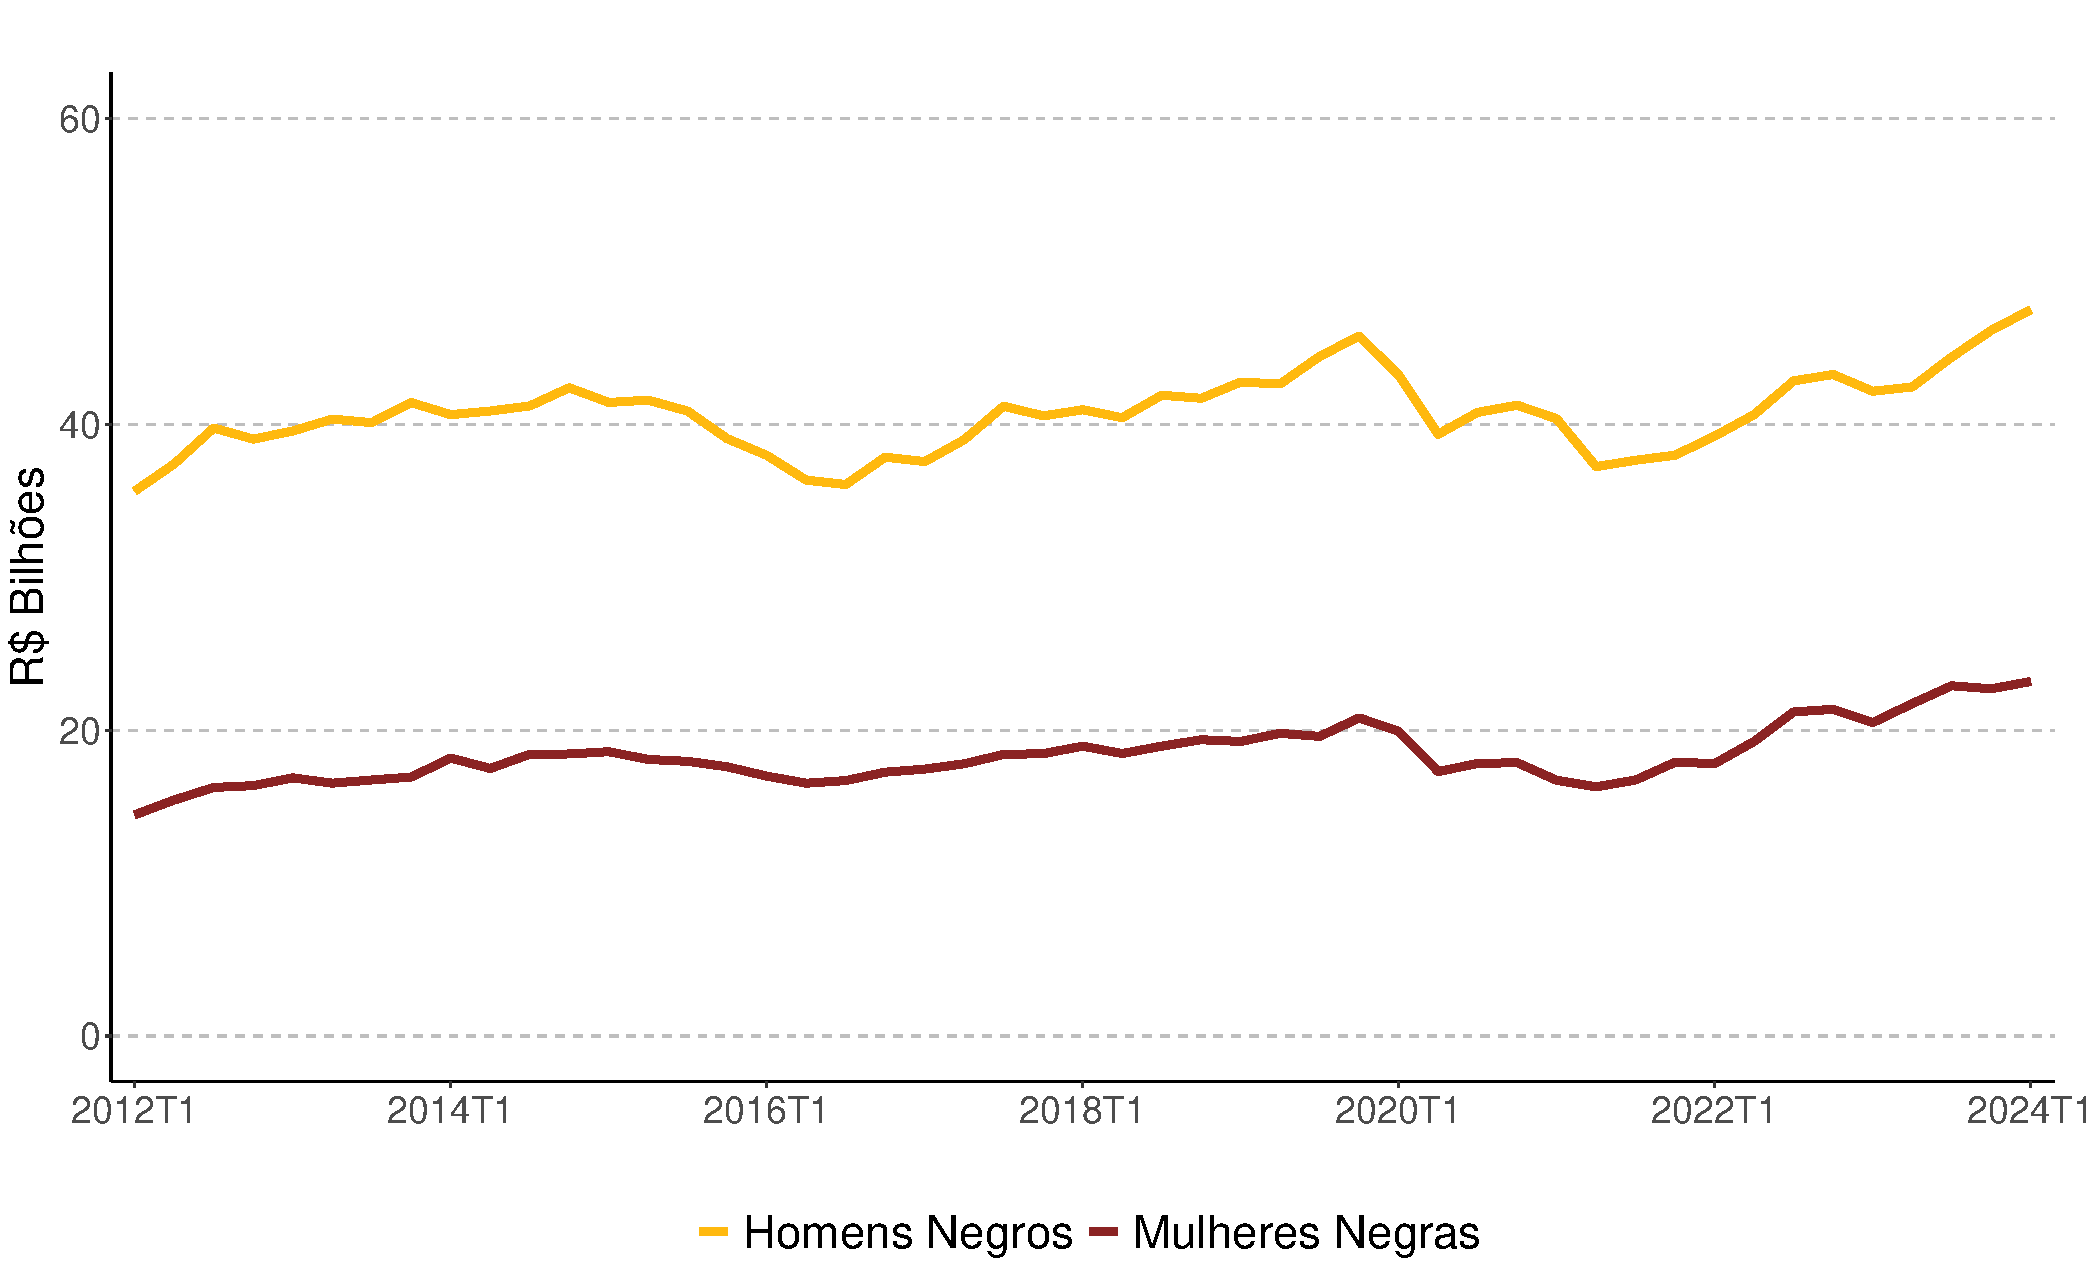
\includegraphics[width = 0.75\textwidth]{figures_output/perda_massa_salarial_composicao.pdf}
	\end{figure}
\end{frame}	

	\begin{frame}{Massa Salarial Perdida - Efeito Discriminação}
	\begin{figure}
		\centering
		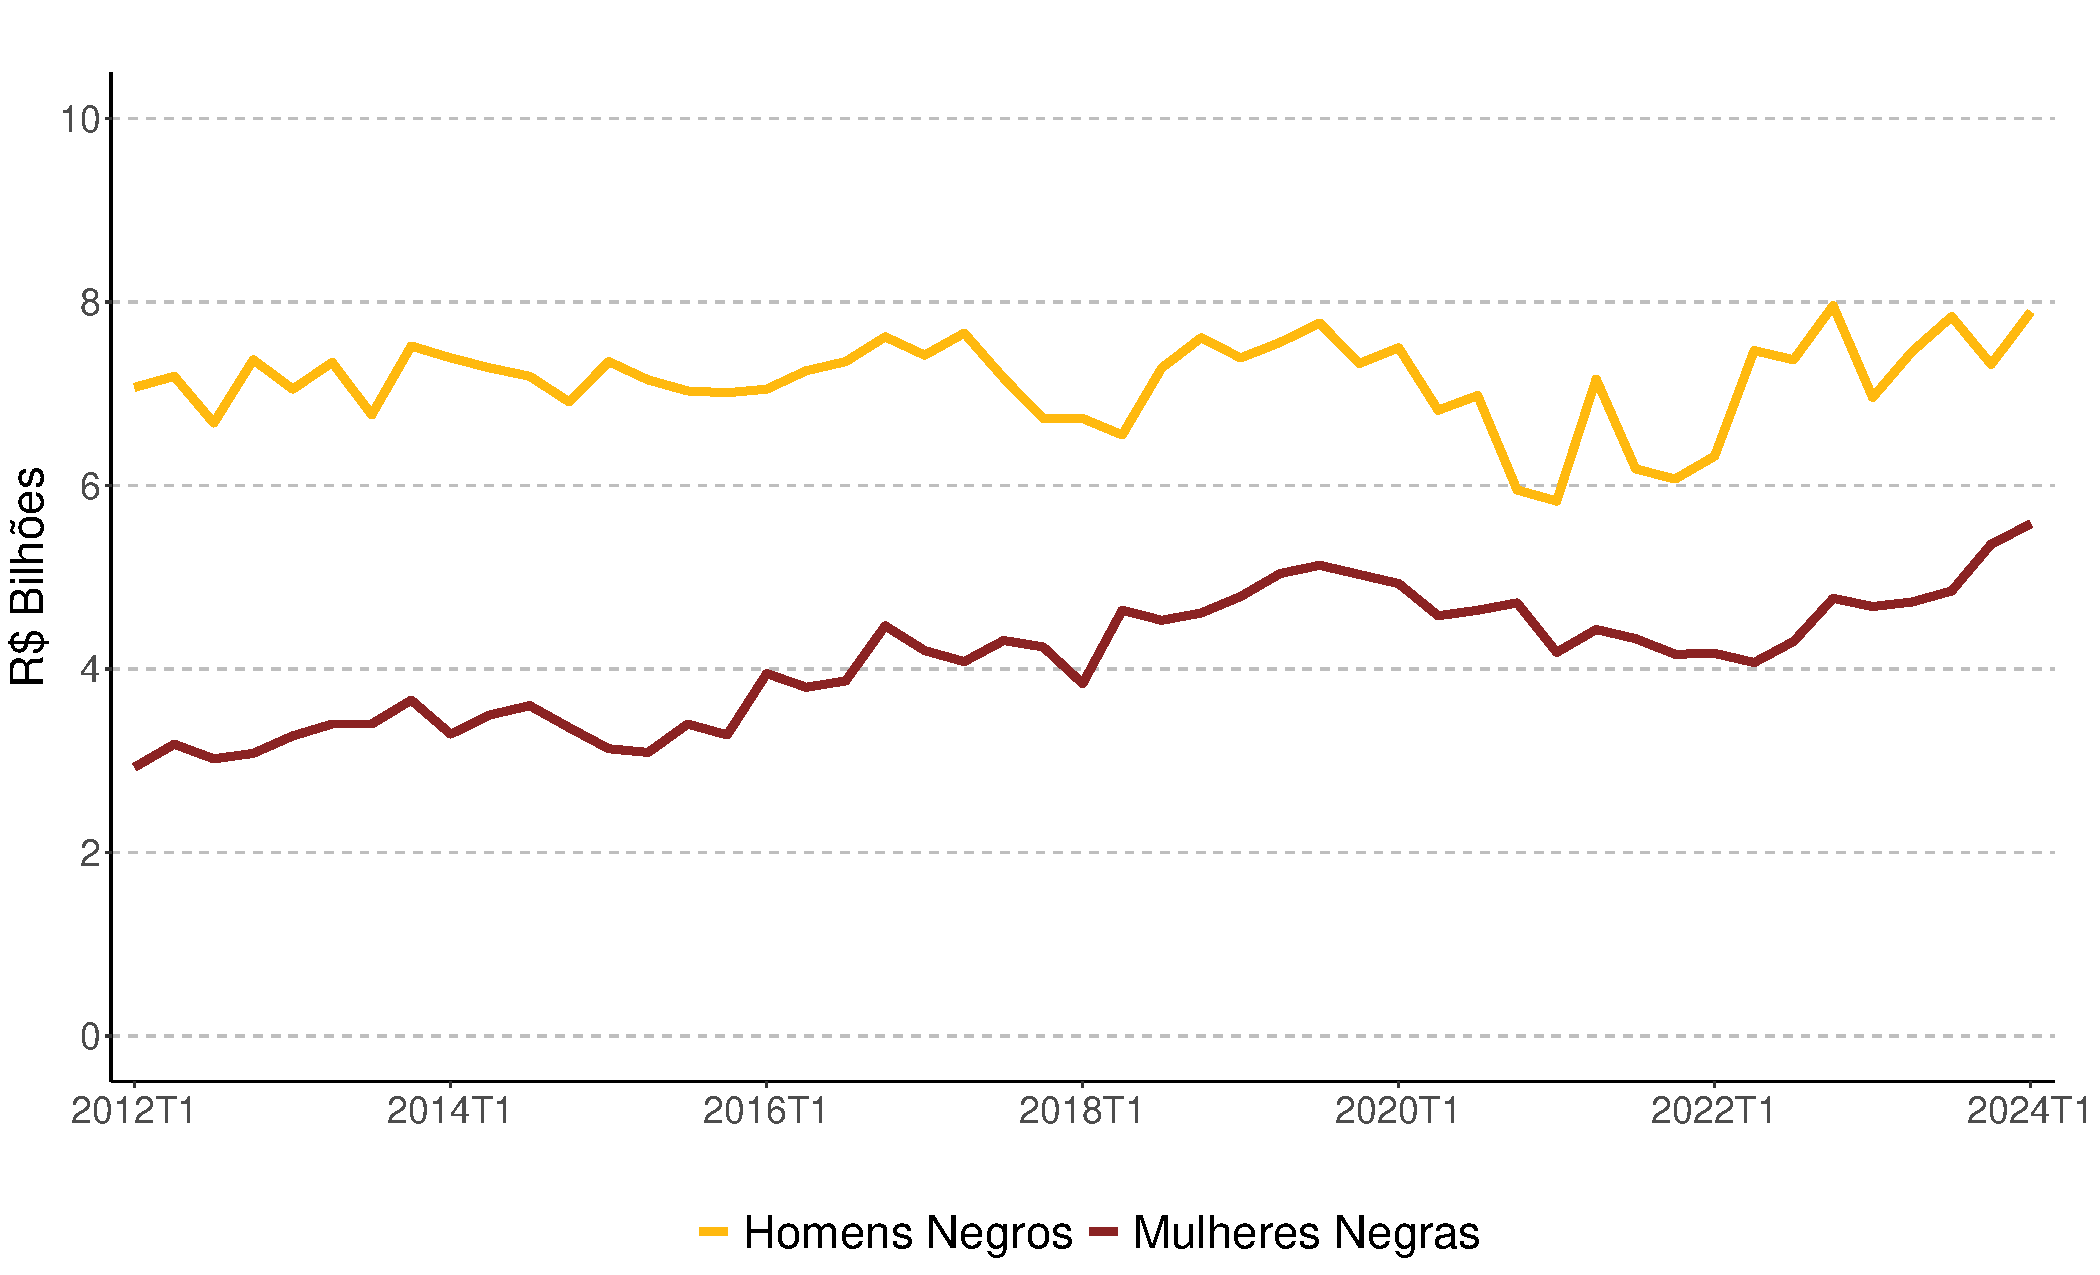
\includegraphics[width = 0.75\textwidth]{figures_output/perda_massa_salario_discriminacao.pdf}
	\end{figure}
	\end{frame}	
	
		\begin{frame}{Massa Salarial Perdida dada as Diferenças no Nível de Empregabilidade }
		\begin{figure}
			\centering
			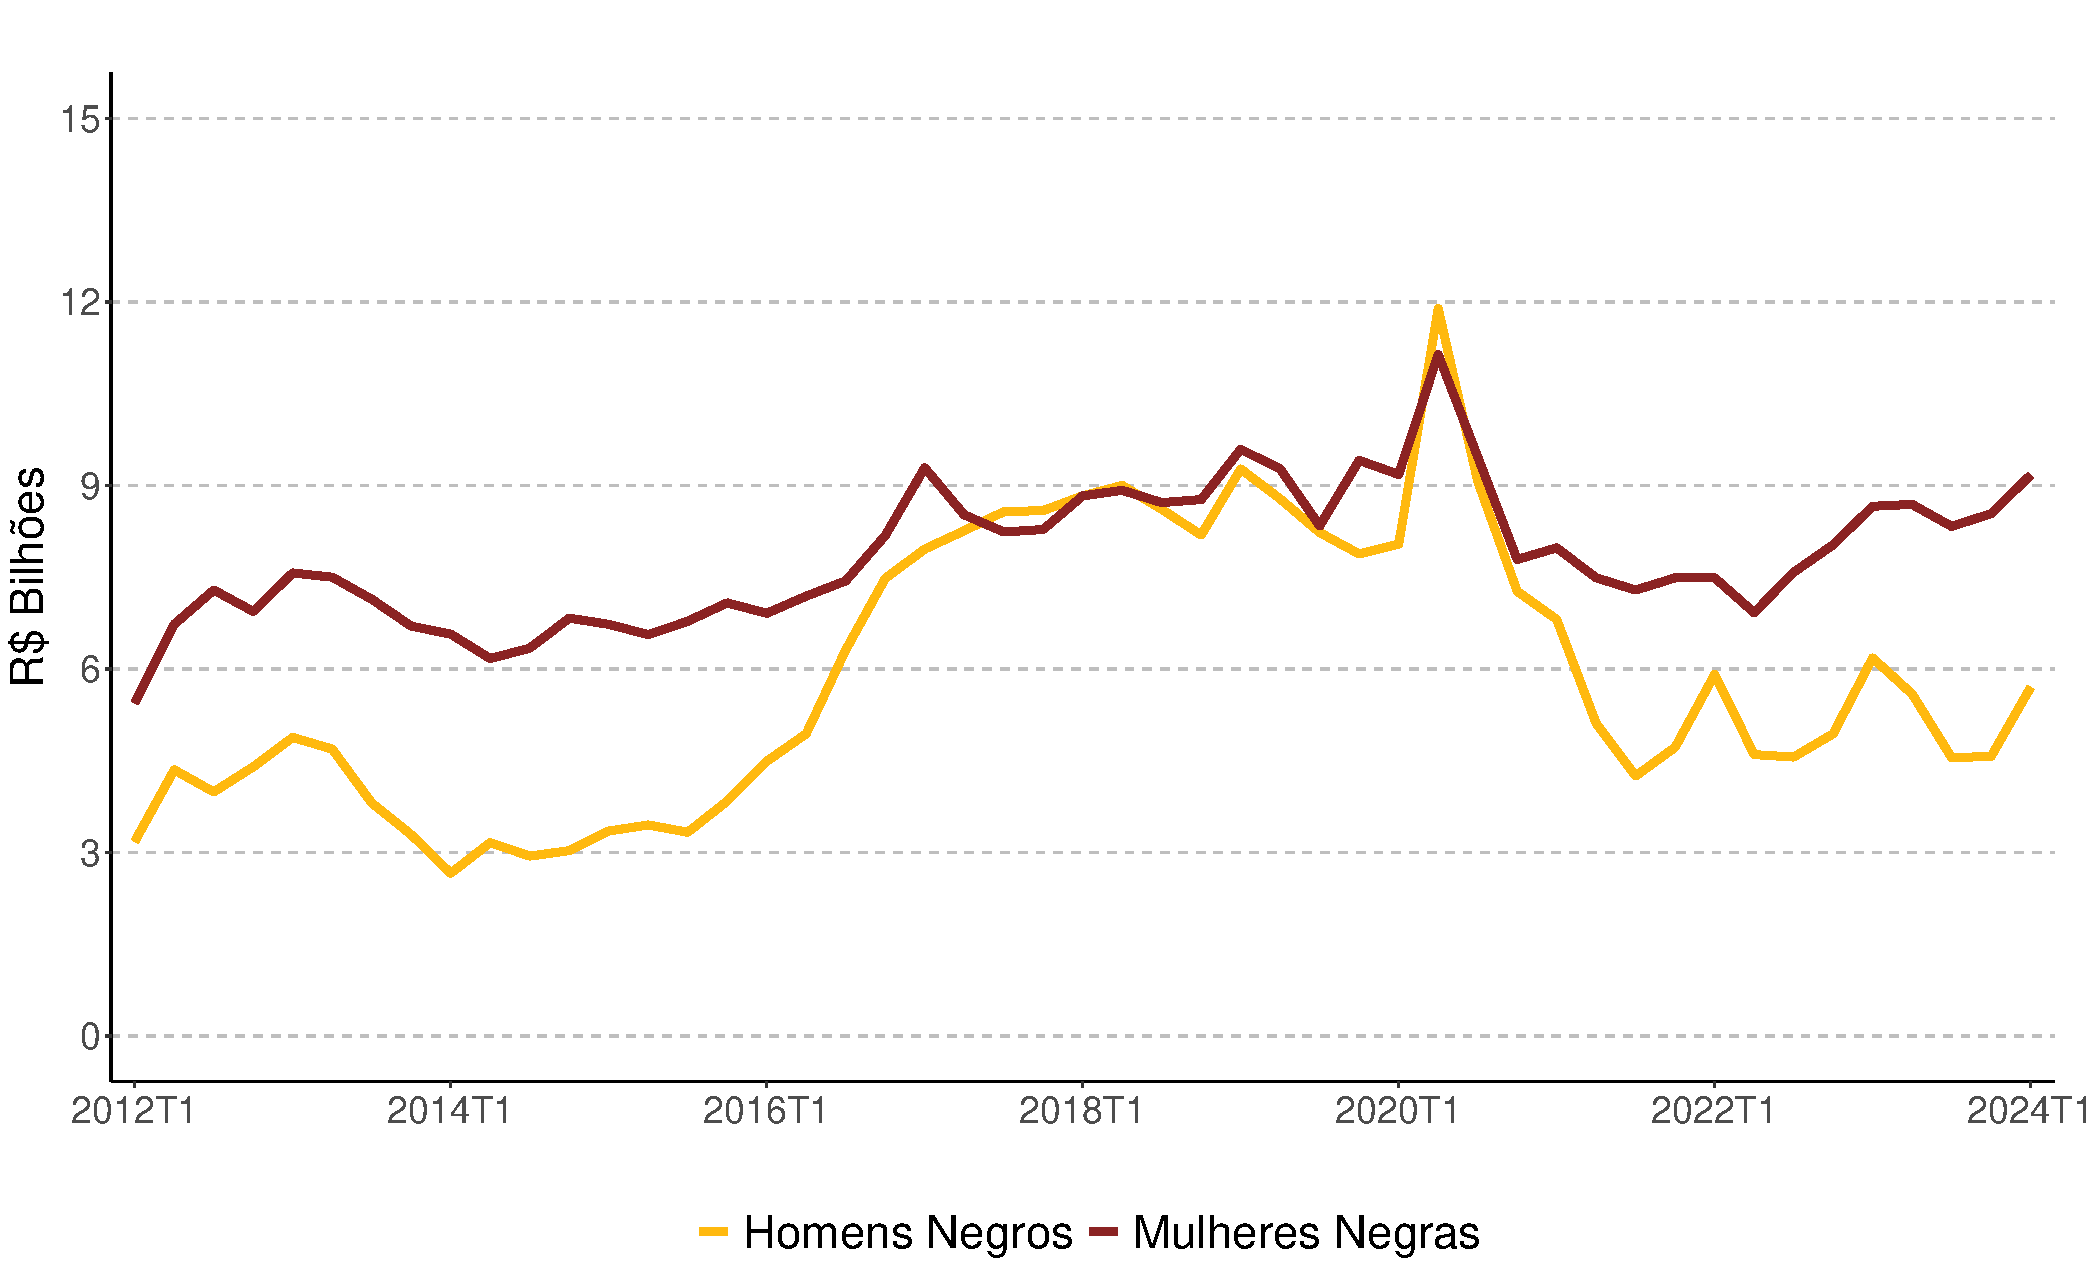
\includegraphics[width = 0.75\textwidth]{figures_output/perda_massa_emp_total.pdf}
		\end{figure}
	\end{frame}	
	
	\begin{frame}{Massa Salarial Perdida dada a Empregabilidade - Efeito Composição}
	\begin{figure}
		\centering
		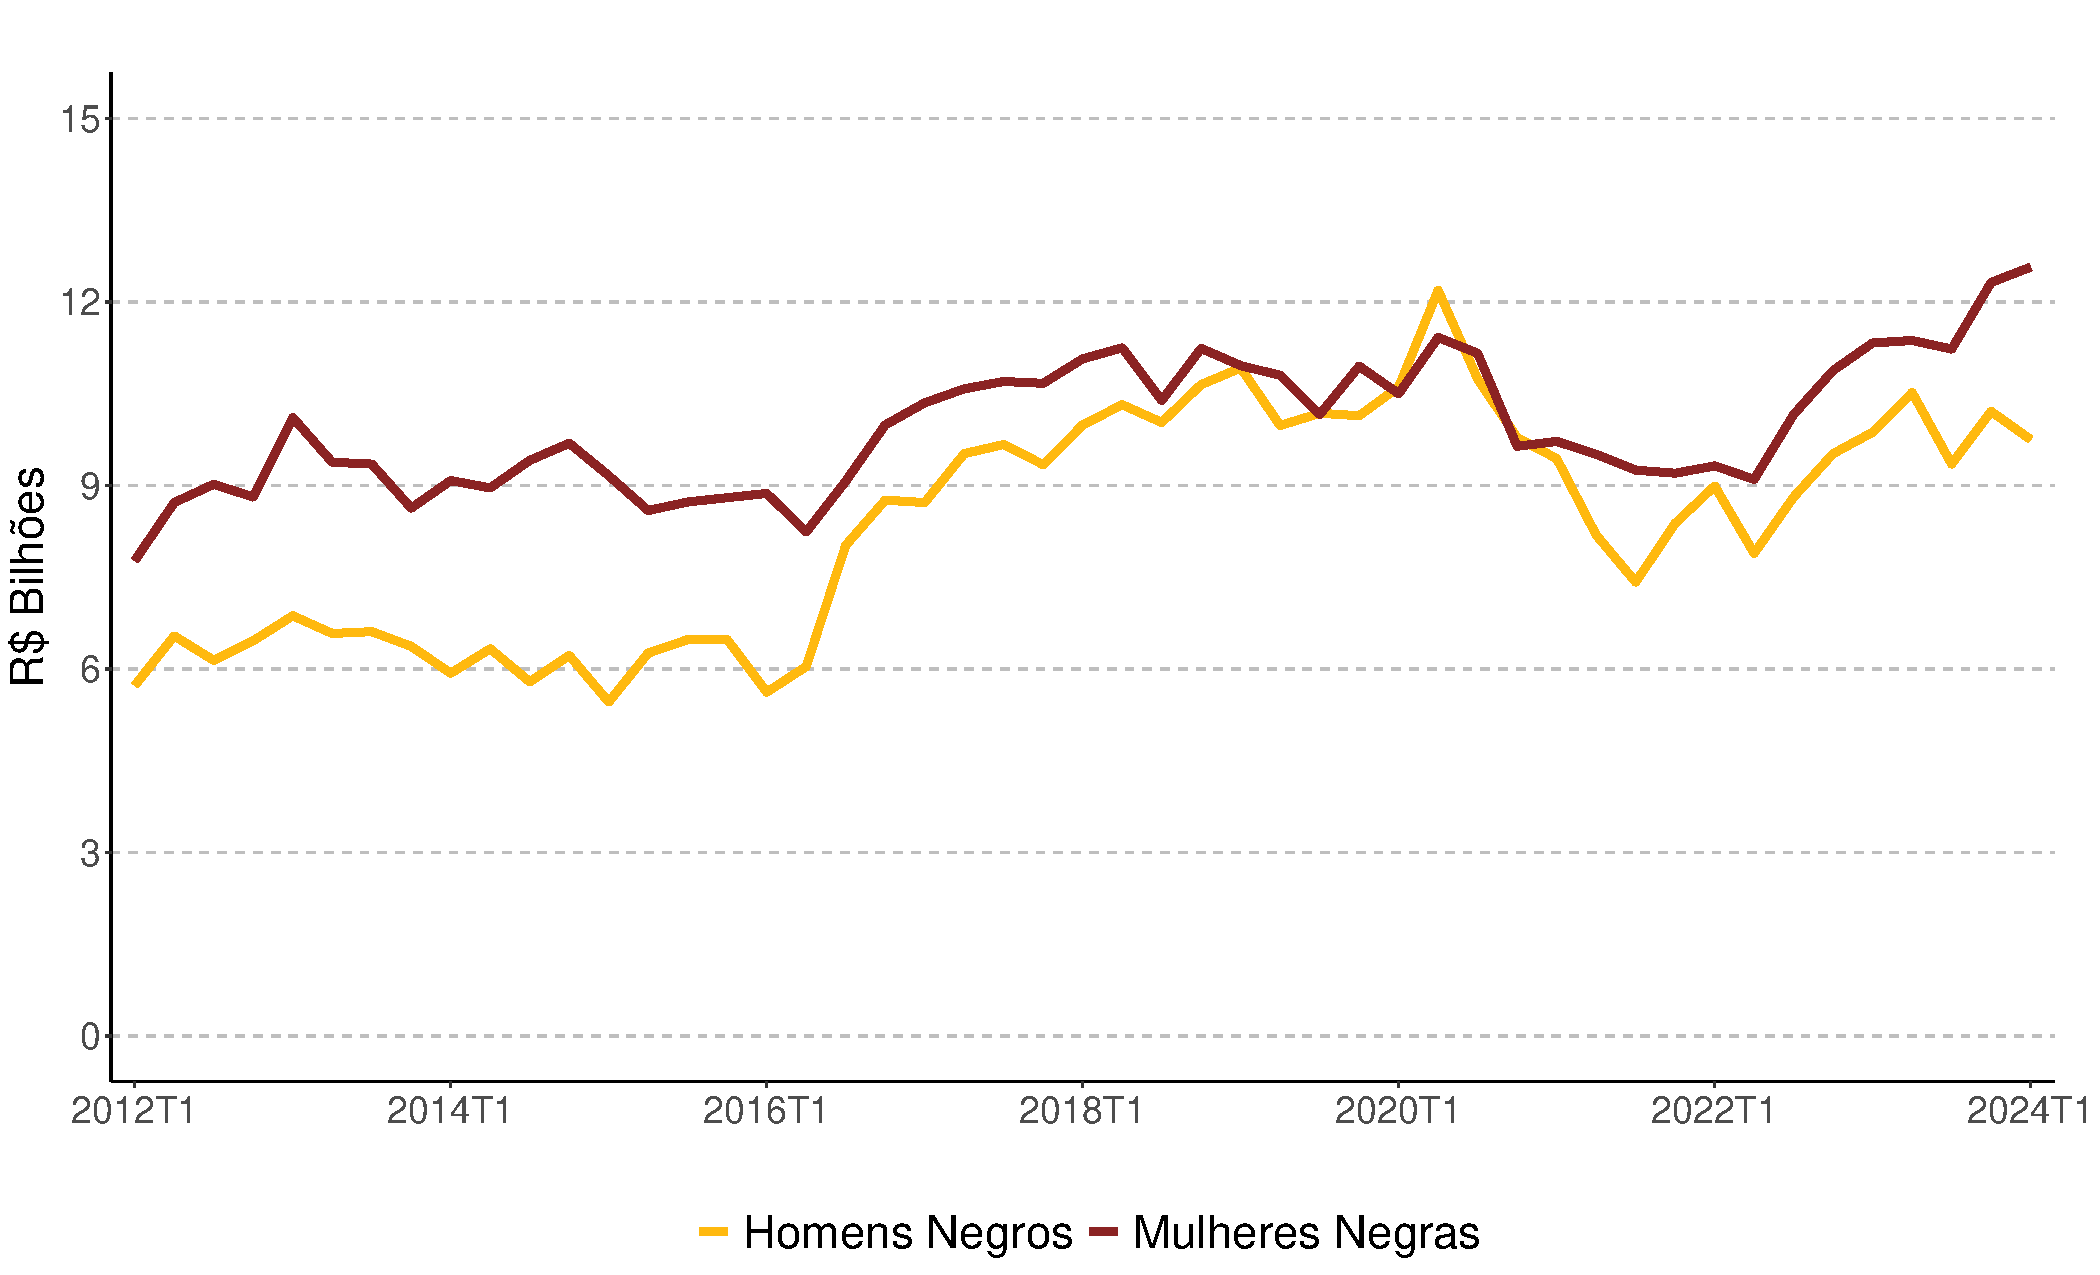
\includegraphics[width = 0.75\textwidth]{figures_output/perda_massa_emp_composicao.pdf}
	\end{figure}
\end{frame}	

	\begin{frame}{Massa Salarial Perdida dada a Empregabilidade - Efeito Discriminação}
	\begin{figure}
		\centering
		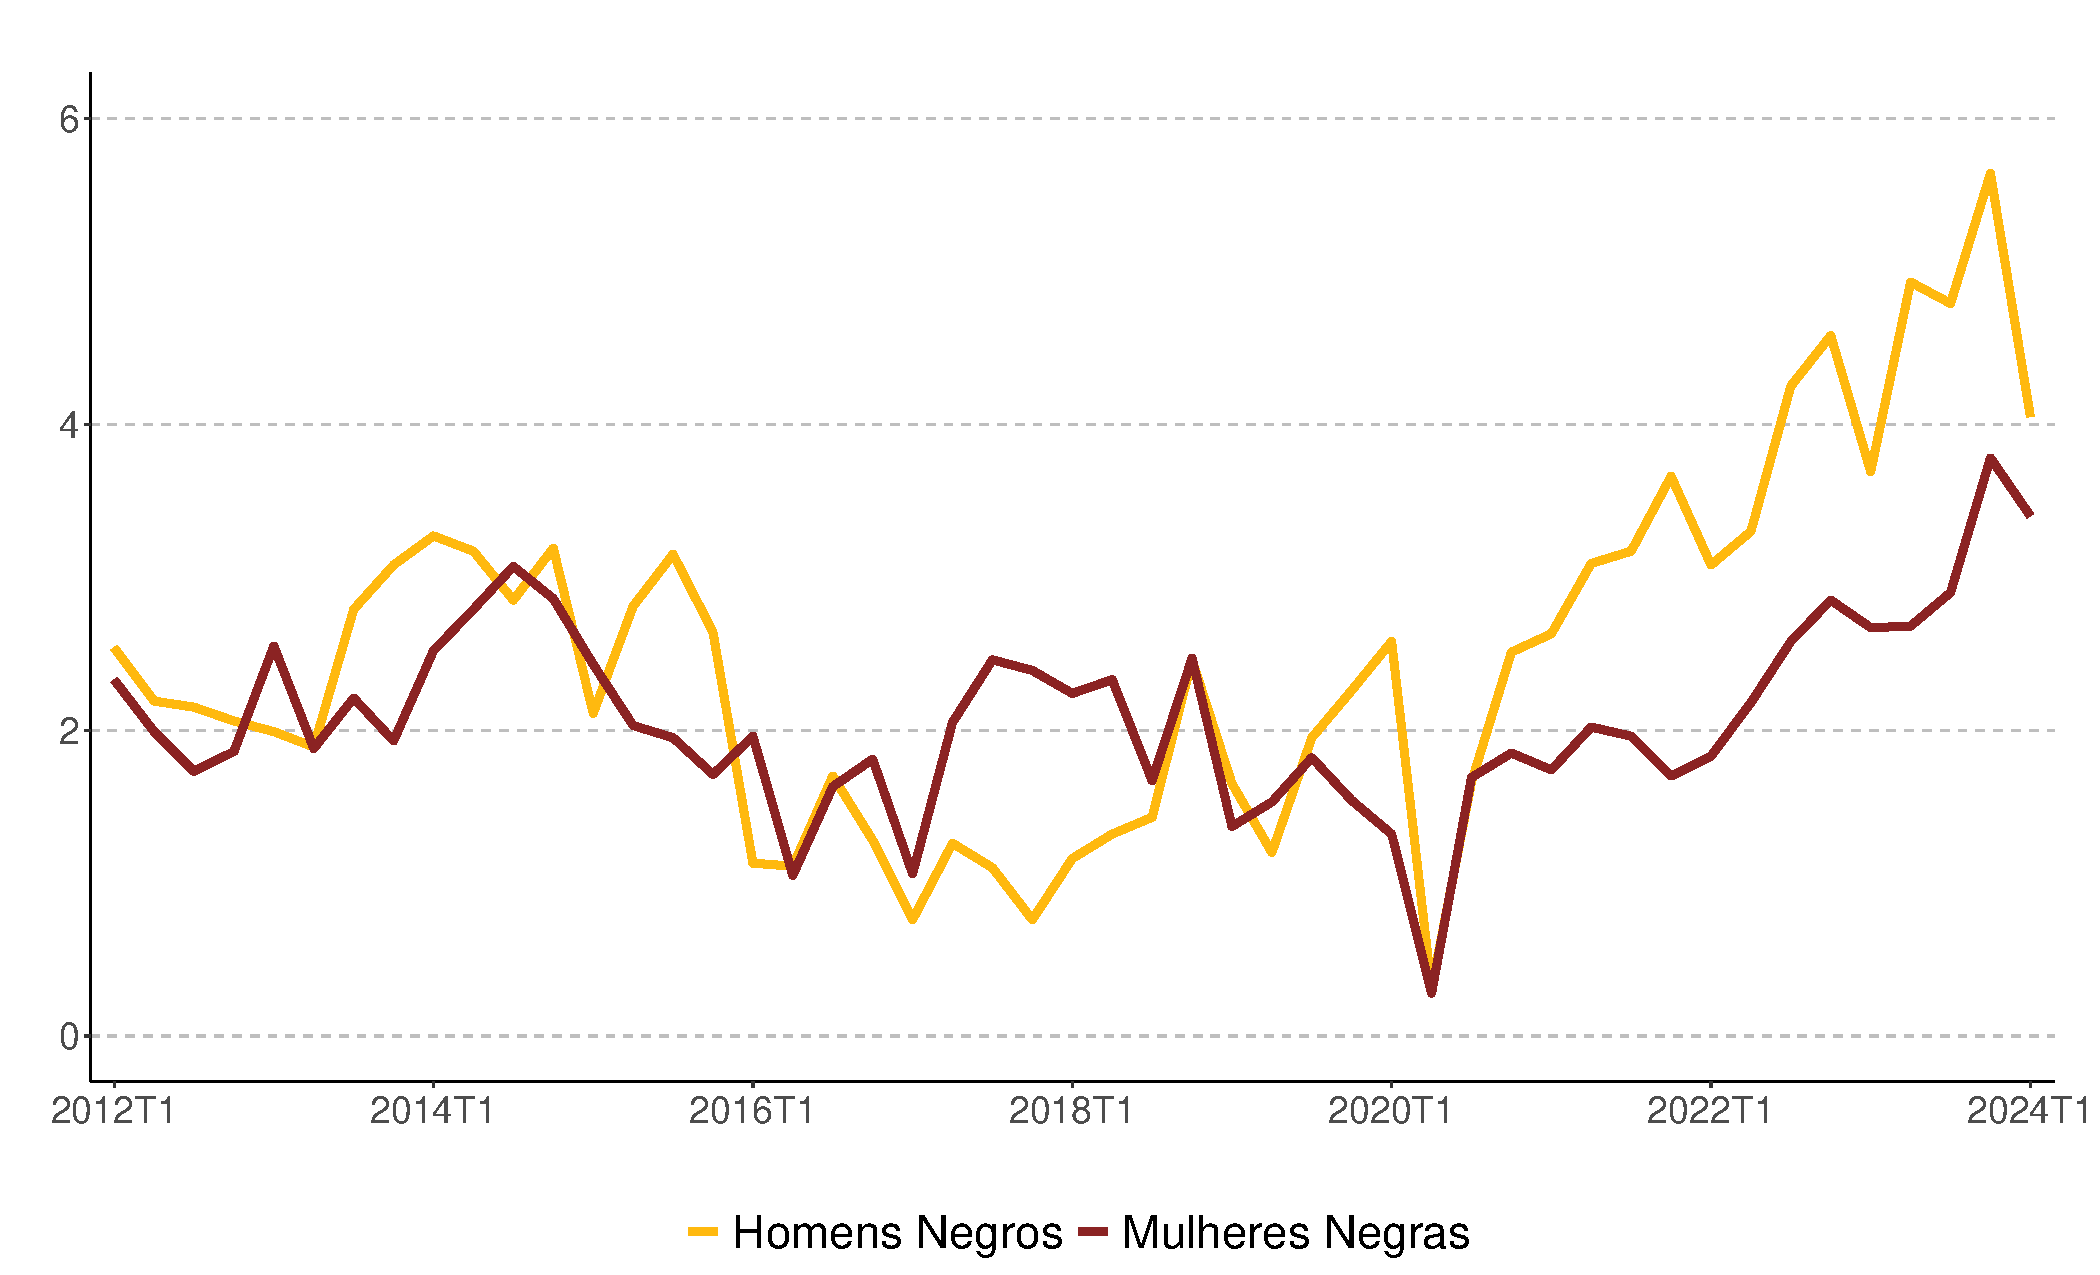
\includegraphics[width = 0.75\textwidth]{figures_output/perda_massa_emp_discriminacao.pdf}
	\end{figure}
\end{frame}	


\end{document}
